\chapter{Context and Related Work}
\label{cha:related_work}
\minitoc

\section{Global Warming and ICT Role}
Global warming is one of the most critical environmental issues of our day \cite{houghton2005global}. Global warming is the effect of human activities on the climate, mainly the burning of fossil fuels (coal, oil, and gas) and large-scale deforestation \cite{houghton2005global}. Both activities have grown immensely since the industrial revolution. The burning of fossil fuels process results in greenhouse gas emissions \cite{olabi2022renewable}. Today, fossil fuels are one of the world's main sources of energy production, emitting more and more GHG \cite{olabi2022renewable}. GHG stays in the atmosphere creating a layer as a blanket over the planet's surface. Without this blanket, the Earth can balance the radiation energy from the sun and the thermal radiation from the Earth to space \cite{houghton2005global}. However, this human-generated blanket imposes a barrier to the thermal radiation from the Earth, heating the planet. All this process works as a greenhouse which is the reason for the name greenhouse gas \cite{houghton2005global}.

This situation brings us to United Nations Climate Change Conference (COP21) in Paris, France, on 12 December 2015. At this conference, 196 parties signed the Paris Agreement aiming to \cite{nations_paris_nodate}:
\begin{enumerate}
    \item Reduce global greenhouse gas emissions substantially, limiting the global temperature increase in this century to 2 \degree C while pursuing measures to limit the growth even further to 1.5 \degree C;
    \item Review countries’ commitments every five years (through the Nationally Determined Contribution, or NDC);
    \item Provide financing to developing countries to mitigate climate change, strengthen resilience, and enhance their abilities to adapt to climate impacts. 
\end{enumerate}

These are ambitious but necessary objectives. Since then, countries and organizations have proposed several actions and pledges. However, a recent report indicates that the actual world's effort is not enough \cite{tracker2022projections}. Figure \ref{fig:ghg_cat} shows GHG emission and temperature estimations. We could see that there is a small reduction in emissions increase tendency. Nevertheless, this figure estimates that real-world actions based on current policies will lead to an increase of somewhere between 2.6 and 2.9 \degree C by 2100. Another recent report confirms the estimation of 2.8 \degree C by 2100 \cite{lee2023ar6}. This estimation is well above the 1.5 \degree C pursued by the Paris Agreement. Considering the targets proposed by the countries through NDC, the temperature will be around 2.4 \degree C. In a scenario based on 2030 NDC targets and submitted and binding long-term targets, the prediction is a temperature of 2 \degree C by 2100, the limit proposed by the Paris Agreement. The report forecasts an optimistic scenario considering the effect of full implementation of all announced targets (e.g., net zero targets) in about 140 countries. Even in this optimistic scenario, the estimated temperature would be 1.8 \degree C. The situation tends to be even worst with the gold rush for gas \cite{tracker2022massive}. The report indicates that in 2022 we arrived at 1.2 \degree C warming \cite{tracker2022projections}.

\begin{figure}[!htb]
    \centering
    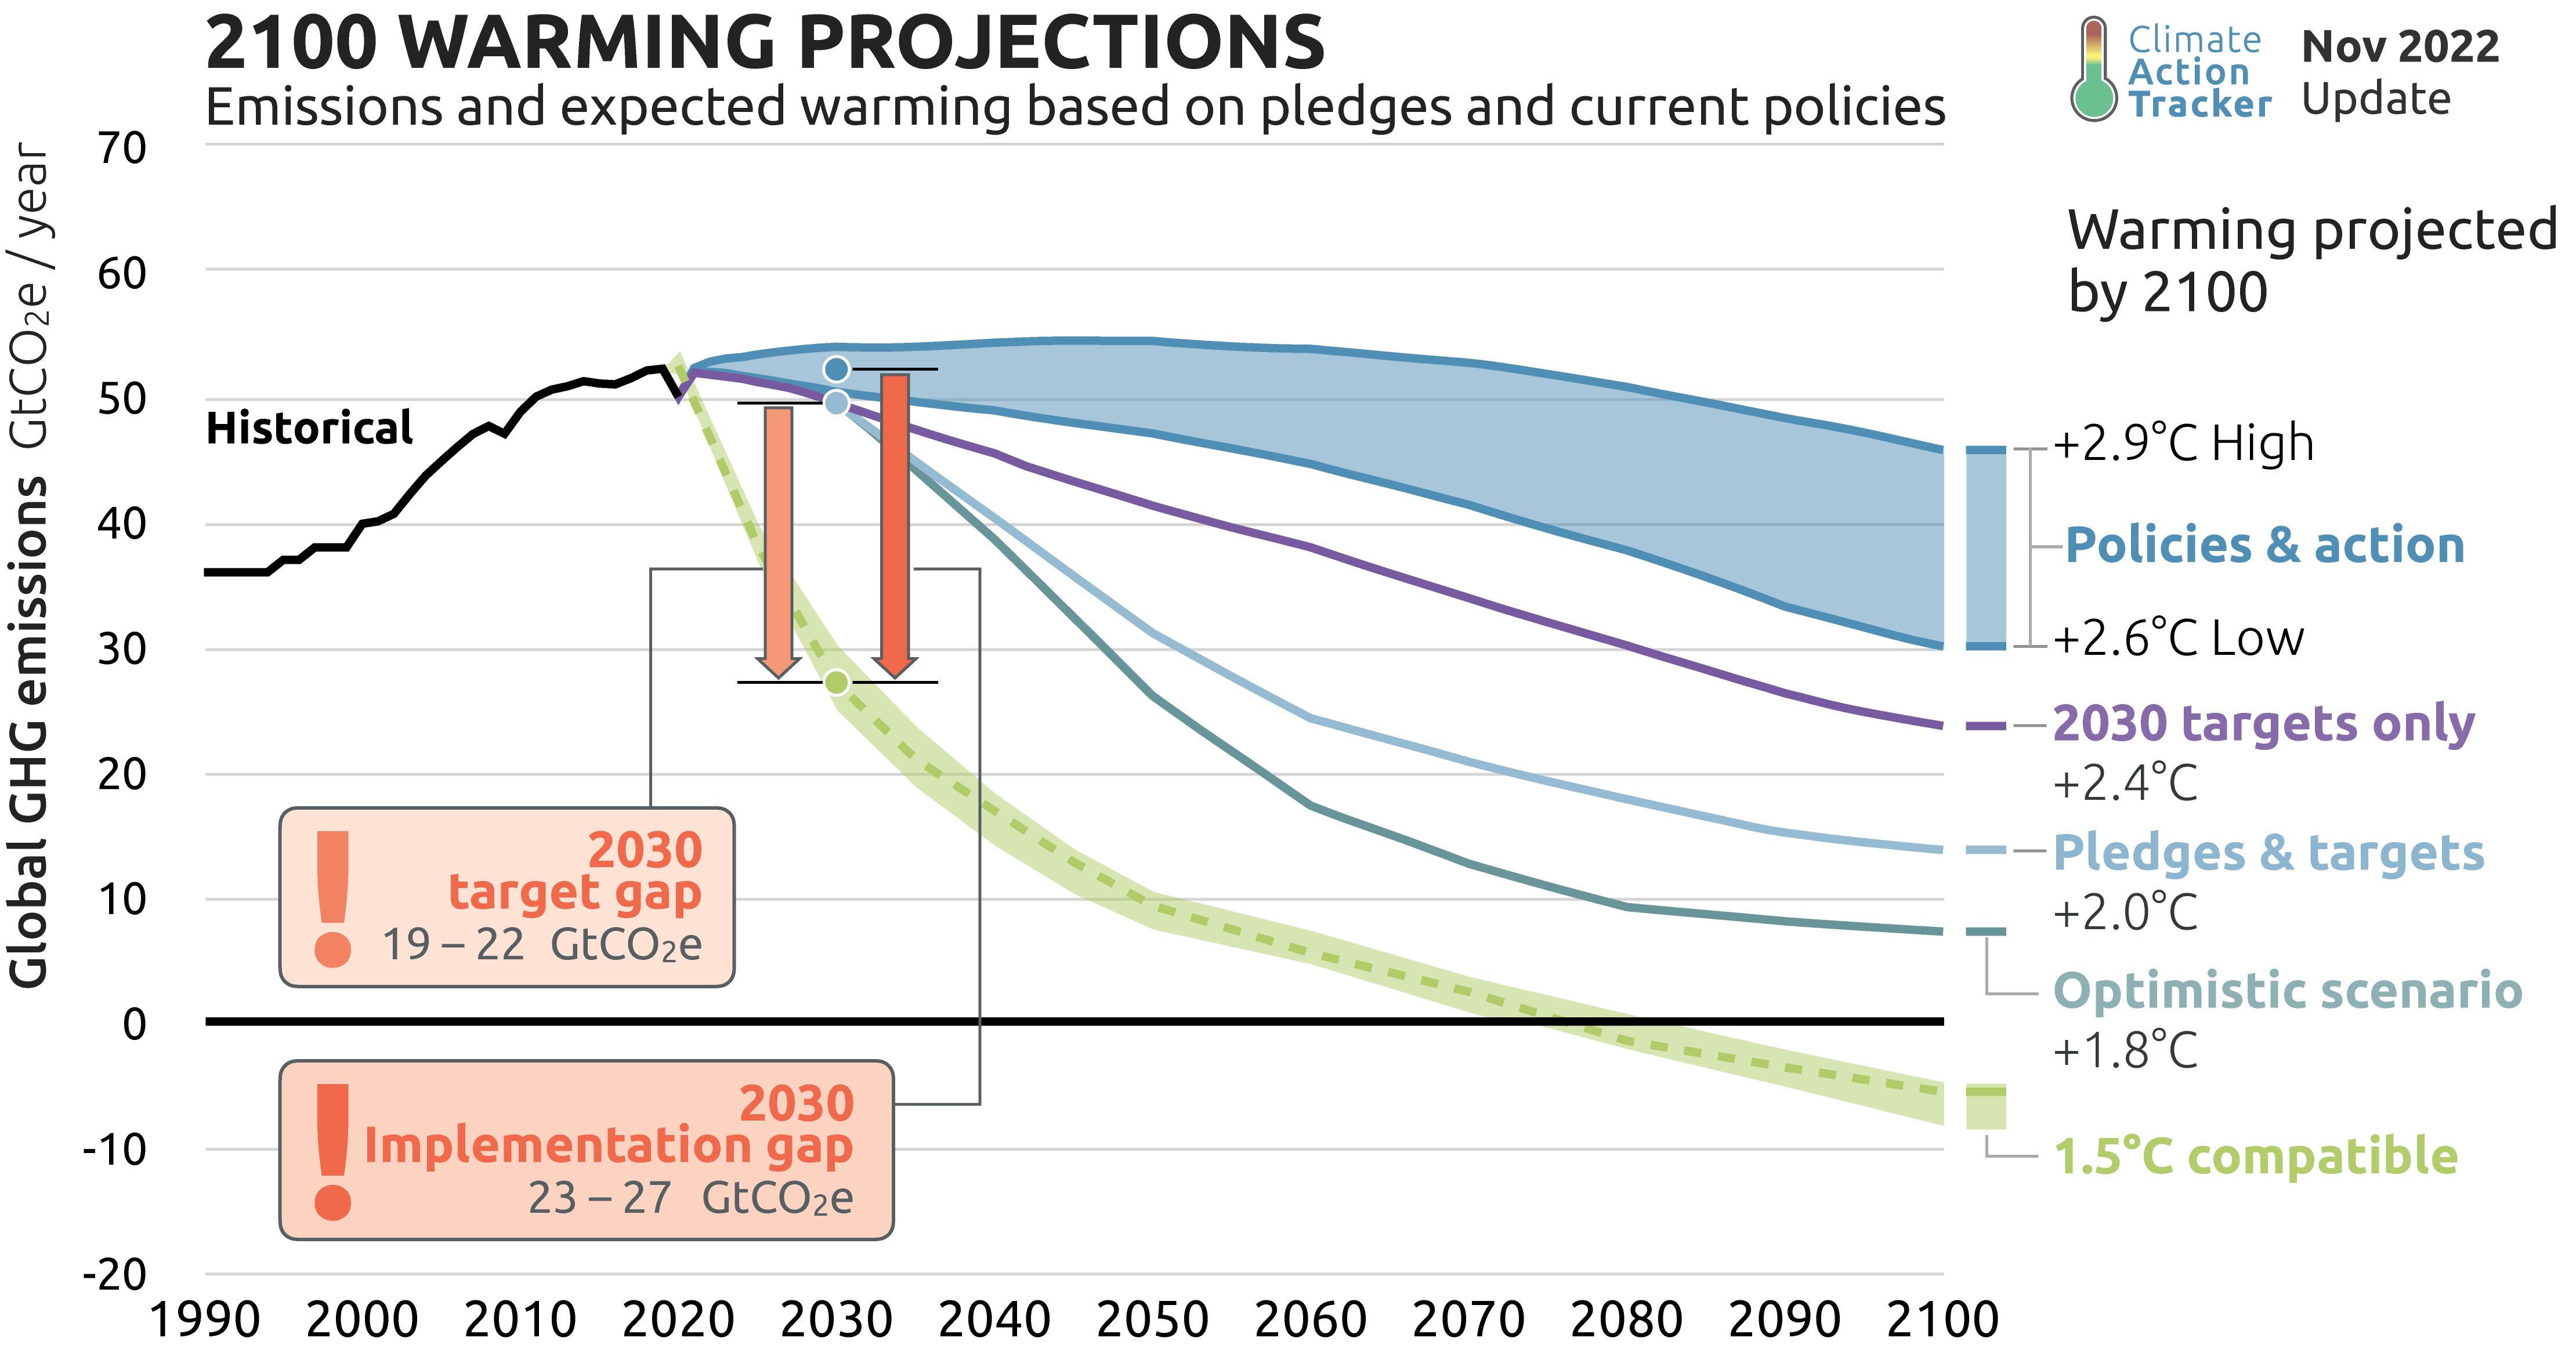
\includegraphics[scale=0.09]{Images/Related_works/Emissions_2022-11.png}
    \caption[Estimated global GHG emissions.]{Estimated global GHG emissions \cite{tracker2022projections}.}
    \label{fig:ghg_cat}
\end{figure}

We have started to feel the impacts of global warming on humanity, such as heatwaves, droughts, and floods, impacting flora and fauna directly \cite{masson2018global, change2022threat}. In a cascade effect, this increases food and water insecurity worldwide \cite{change2022threat, doi:10.1126/science.1239402}. In addition, high temperatures increase mortality, impact labor productivity, impair learning, increase adverse pregnancy outcomes possibility, increase conflict, hate speech, migration, and infectious disease spread \cite{lenton2023quantifying}. Therefore, an increase of the temperature by 2.7 \degree C as forecasted would impact one-third (22–39\%) of the world's population by 2100 \cite{lenton2023quantifying}. Climate change has already impacted around 9\% of people (>600 million) \cite{lenton2023quantifying}. Reducing global warming from 2.7 to 1.5 \degree C results in a $\sim$5-fold decrease in the population exposed to unprecedented heat (mean annual temperature $\geq$29 \degree C) \cite{lenton2023quantifying}. Thus, all sectors must reduce their GHG emissions as much as possible.

Information and Communication Technology is one of these sectors which has accelerated growth in the last 70 years. Unesco defines ICT as \cite{unesco2009guide}:

\begin{quote}
    ``Information and communication technologies (ICT) is defined as a diverse set of technological tools and resources used to transmit, store, create, share or exchange information. These technological tools and resources include computers, the Internet (websites, blogs, and emails), live broadcasting technologies (radio, television, and webcasting), recorded broadcasting technologies (podcasting, audio and, video players, and storage devices), and telephony (fixed or mobile, satellite, visio/video-conferencing, etc.).''
\end{quote}

Regarding the ICT role in GHG emissions, the global share is around 1.8\%-2.8\%, or 2.1\%-3.9\% considering the supply chain pathways in 2020 \cite{freitag2021climate}. The situation tends to get even worst, driven by the boom in Internet-connected devices. A Cisco report indicates that the Internet had 3.9 billion users in 2018 \cite{cisco2020cisco}. The same report predicts an increase to 5.3 billion in 2023 (66 percent of the global population). Furthermore, they predicted 3.6 networked devices per capita in 2023, up from 2.4 networked devices per capita in 2018. However, International Telecommunication Union (ITU), a United Nations specialized agency for ICTs, indicates that we arrived at 5.3 billion connected users in 2022 due to the COVID-19 pandemic \cite{ITU2022}. But will the growth in internet users increase GHG emissions? Andrae and Edler \cite{andrae2015global} and Belkhir and Elmeligi \cite{belkhir2018assessing} agree that this growth could lead to an increase in GHG emissions. Figure \ref{fig:projections_ICT} shows the predictions of both works.

\begin{figure}[!htb]
    \centering
    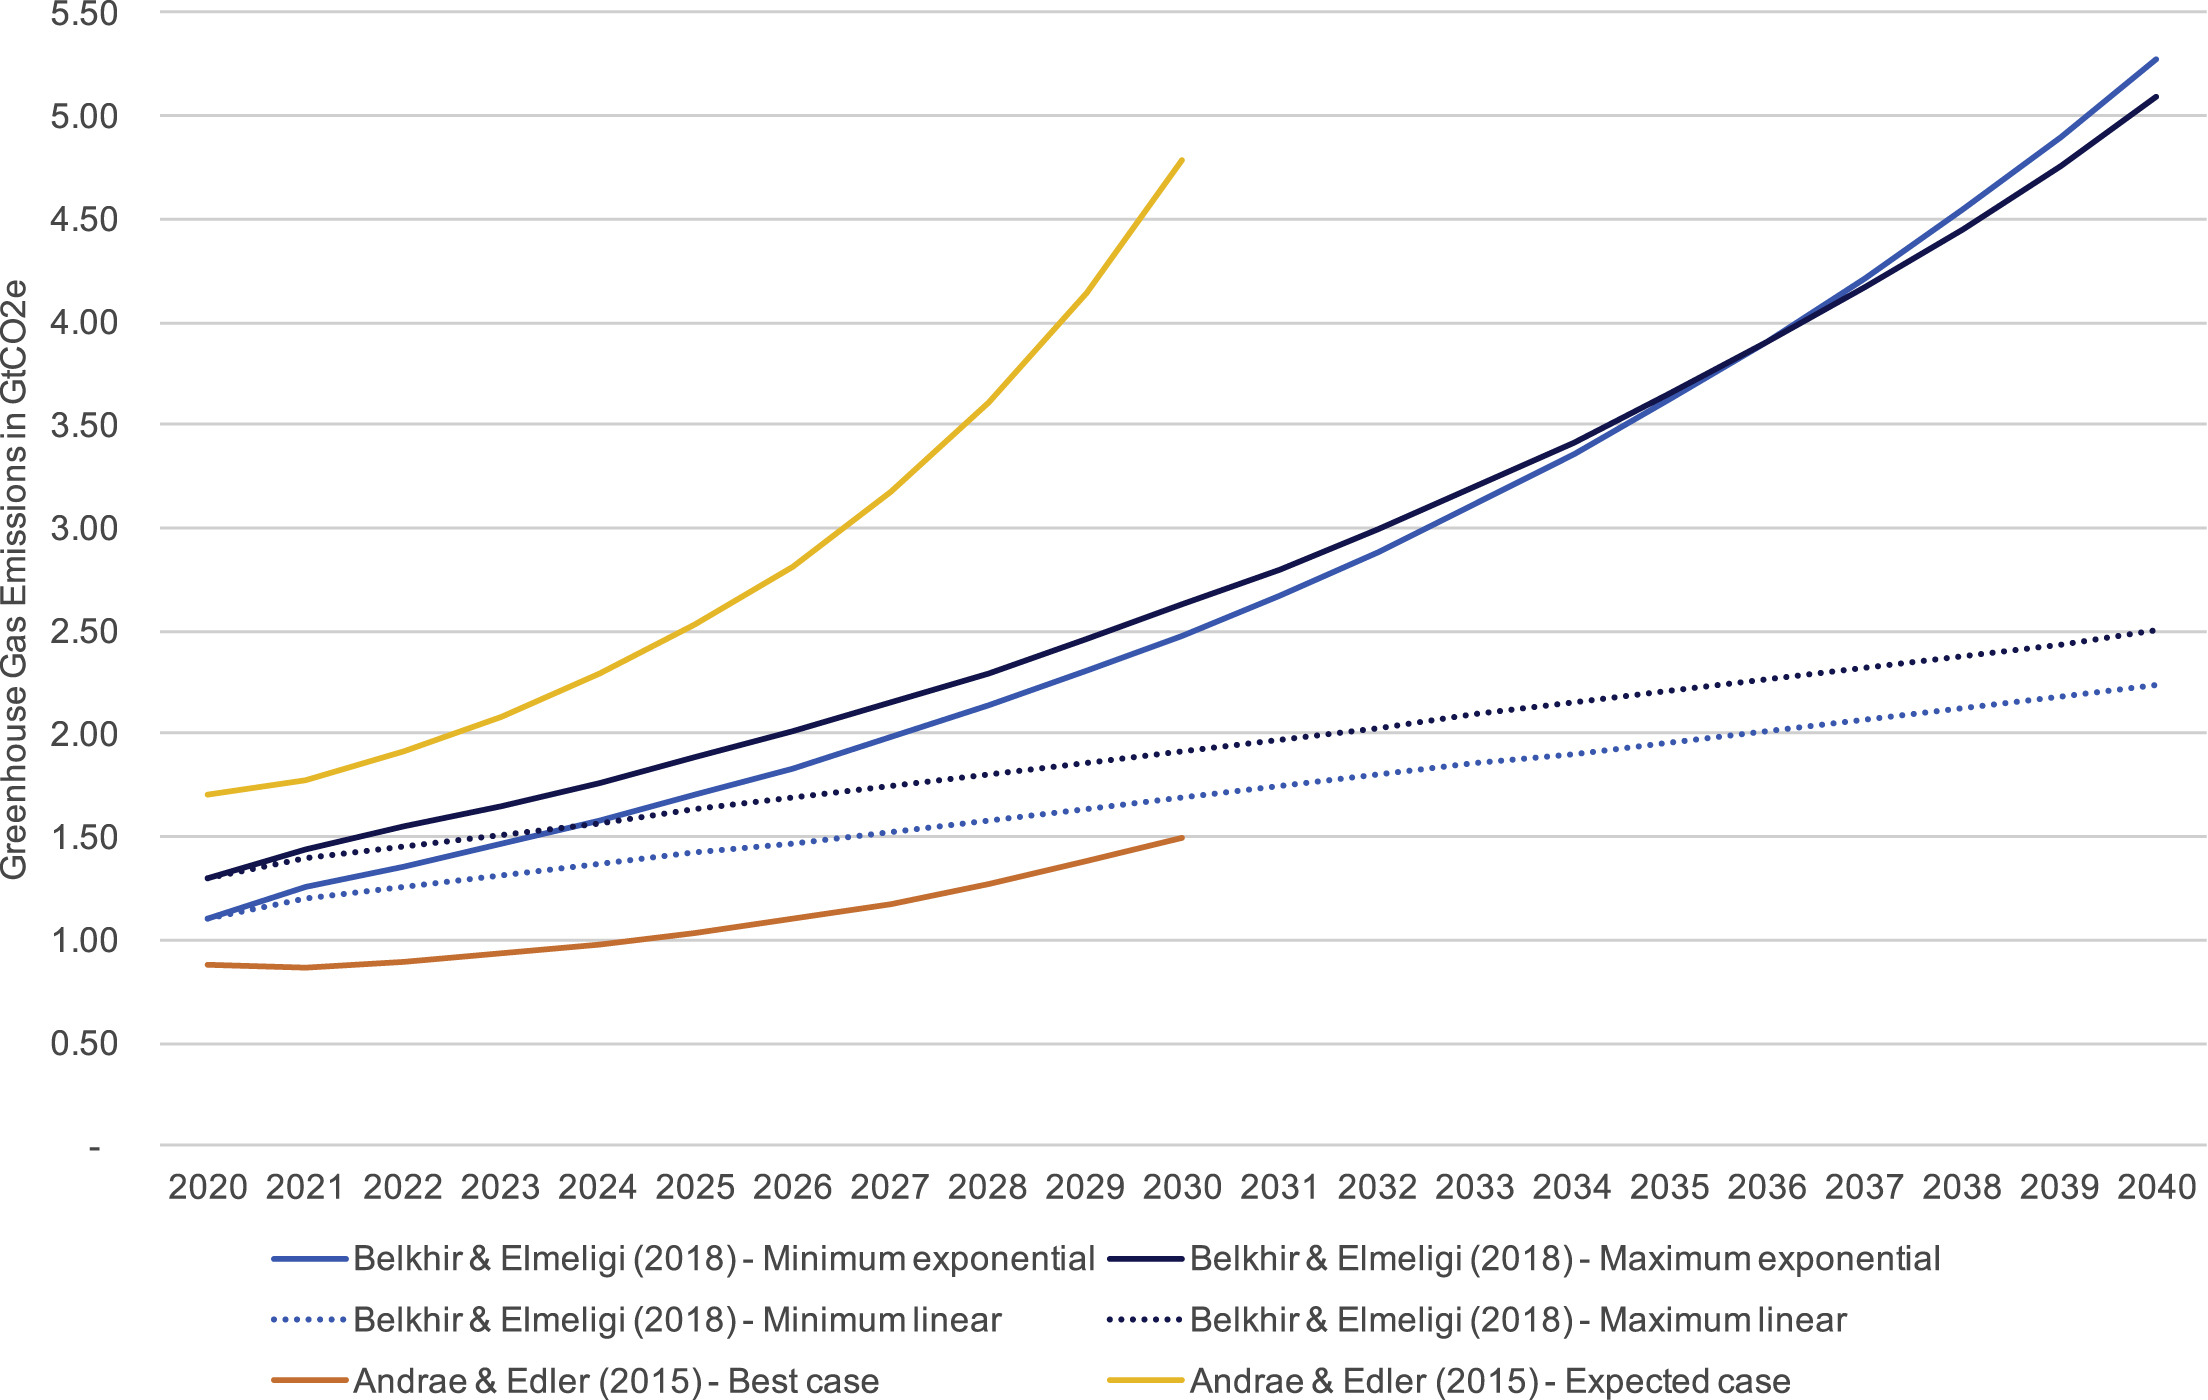
\includegraphics[scale=1]{Images/Related_works/gr4_lrg.jpg}
    \caption[Projections of ICT's GHG emissions from 2020.]{Projections of ICT's GHG emissions from 2020 \cite{freitag2021climate}.}
    \label{fig:projections_ICT}
\end{figure}

This figure illustrates the contraction in the Paris Agreement targets (see Figure \ref{fig:ghg_cat}) and the predictions about usage in the ICT sector. In all forecasts of Figure \ref{fig:projections_ICT}, the tendency is the growth of emissions. However, ICT needs to reduce its emissions drastically. Figure \ref{fig:stable_emissions_ICT} illustrates the carbon emission share if the ICT stays at the same level as 2020 and the other sectors decrease their emissions. Without changes, ICT would have 35.1\% of global emissions in 2050. So, ICT must move towards reducing its emissions. 
% Figure \ref{fig:estimations_ICT} presents the estimations of ICT's GHG emissions for 2015 and 2020 from different authors. This figure breaks down these emissions into different components. 
One of the biggest GHG emitters inside the ICT sector is data centers \cite{freitag2021climate}. IBM defines the data center as ``a physical room, building or facility that houses IT infrastructure for building, running, and delivering applications and services, and for storing and managing the data associated with those applications and services'' \cite{datacenterIBM}. The International Energy Agency (IEA) defines data center as \cite{centres2022data}:
\begin{quote}
    ``Data centers are facilities used to house networked computer servers that store, process and distribute large amounts of data. They use energy to power both the IT hardware (e.g., servers, drives, and network devices) and the supporting infrastructure (e.g., cooling equipment).''
\end{quote}

\begin{figure}[!htb]
    \centering
    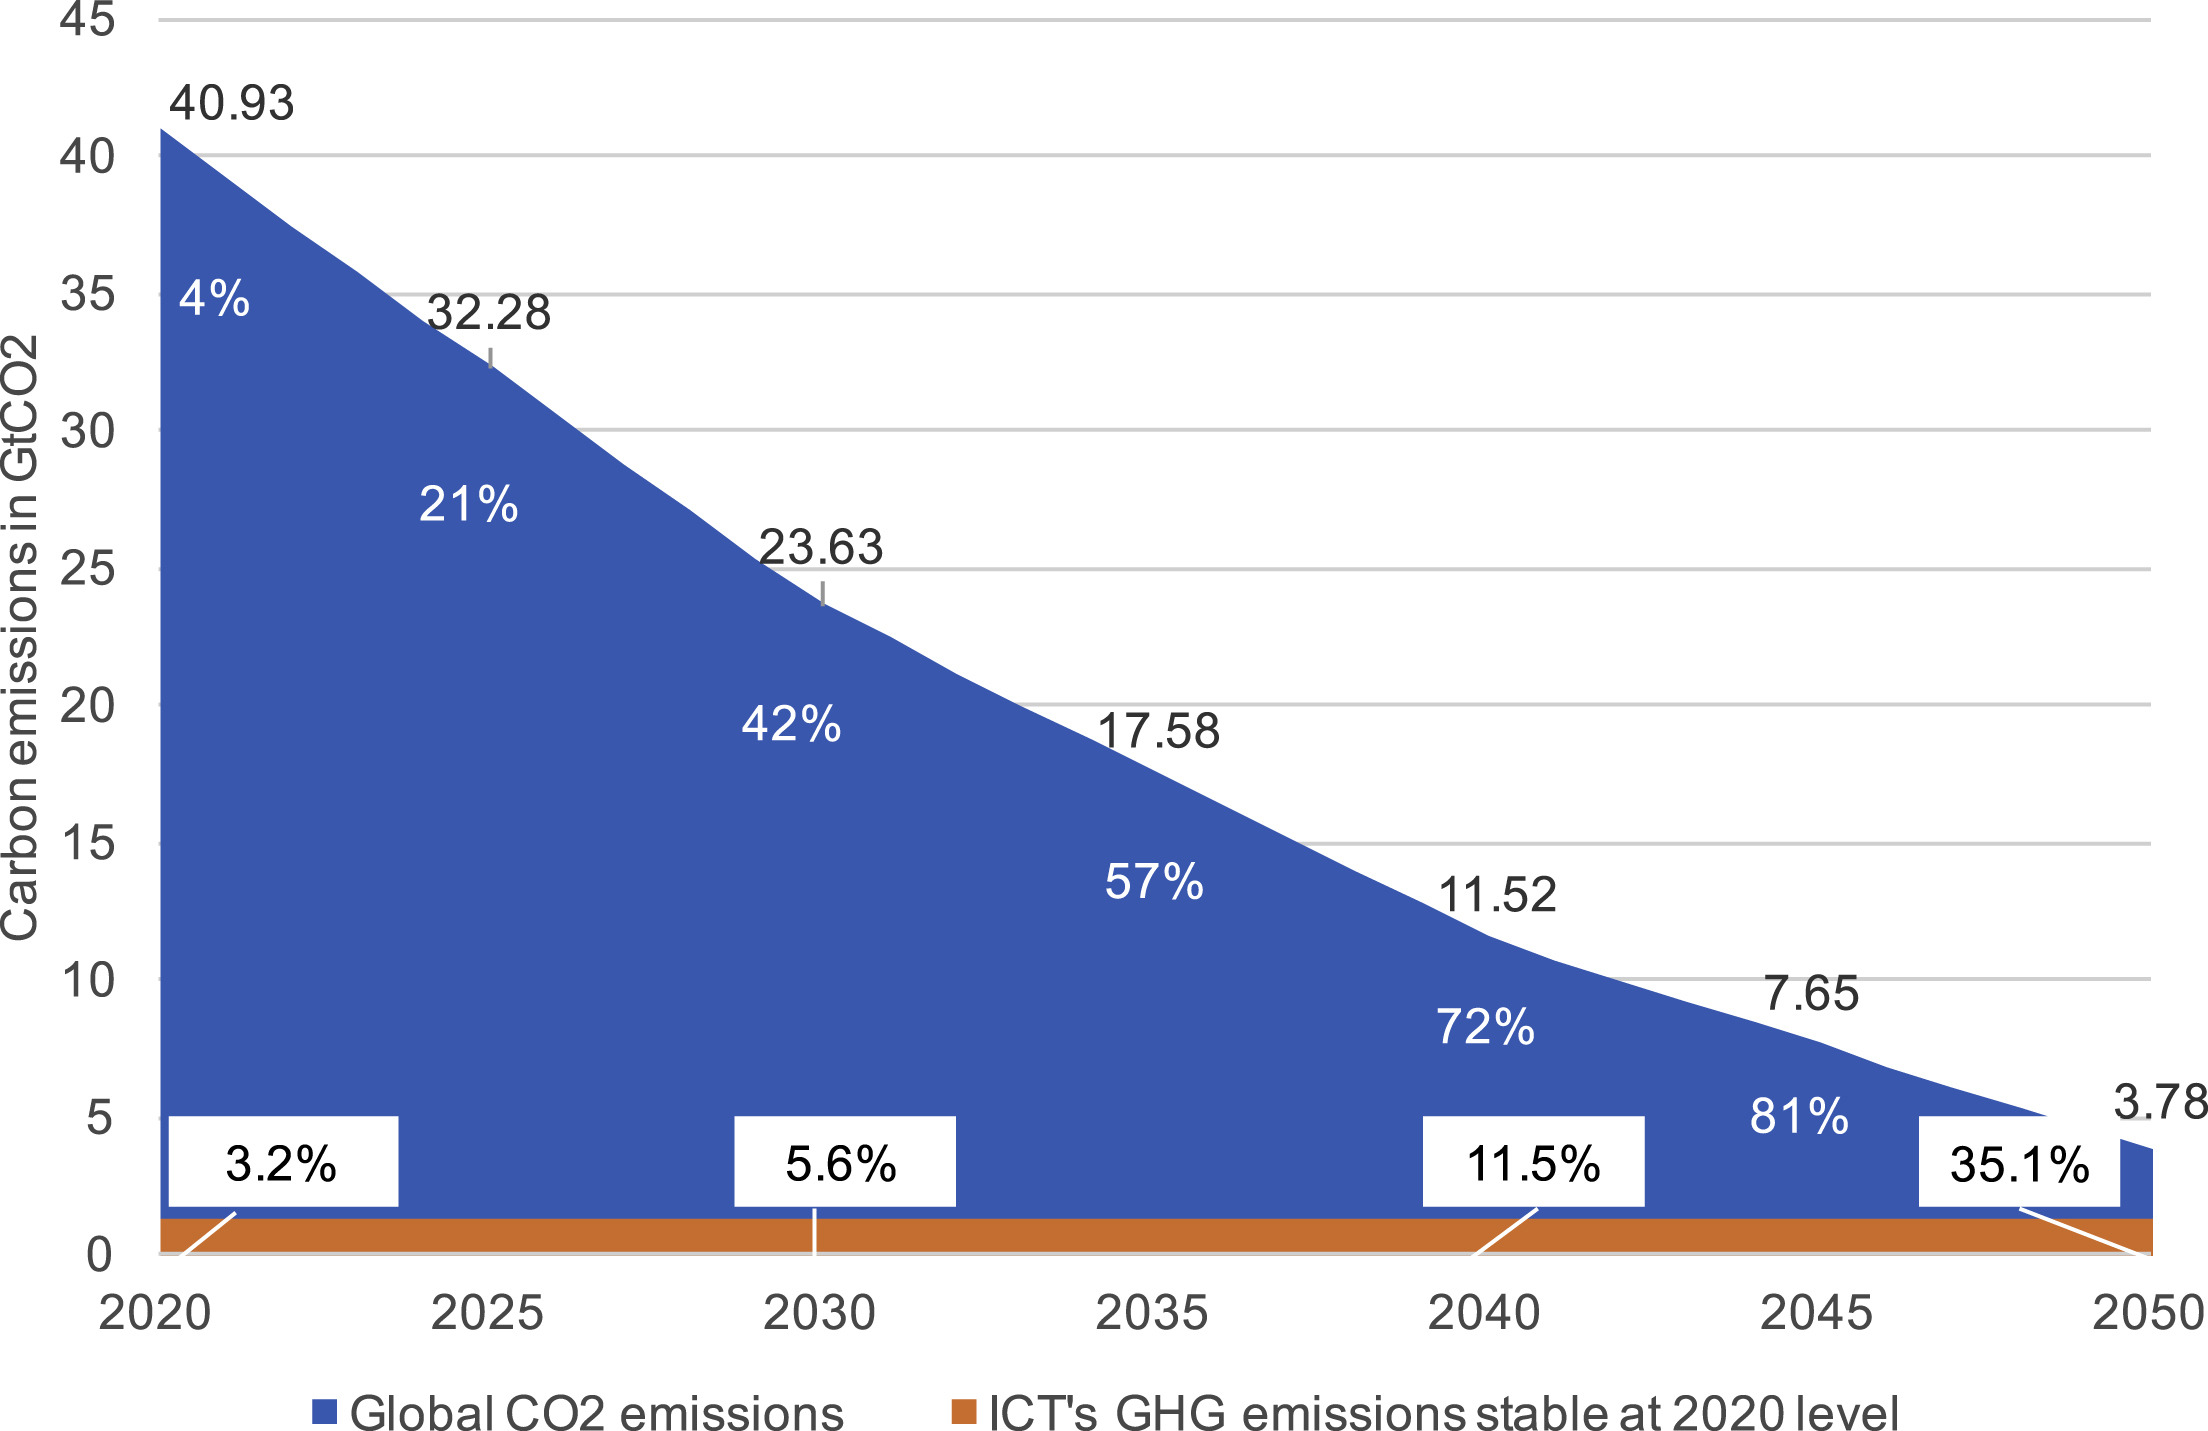
\includegraphics[scale=0.8]{Images/Related_works/gr6_lrg.jpg}
    \caption[ICT's emissions, assuming the 2020 level remains stable until 2050, and global CO2 emissions reduced in line with 1.5 \degree C.]{ICT's emissions, assuming the 2020 level remains stable until 2050, and global CO2 emissions reduced in line with 1.5 \degree C \cite{freitag2021climate}.}
    \label{fig:stable_emissions_ICT}
\end{figure}

% \begin{figure}[!htb]
%     \centering
%     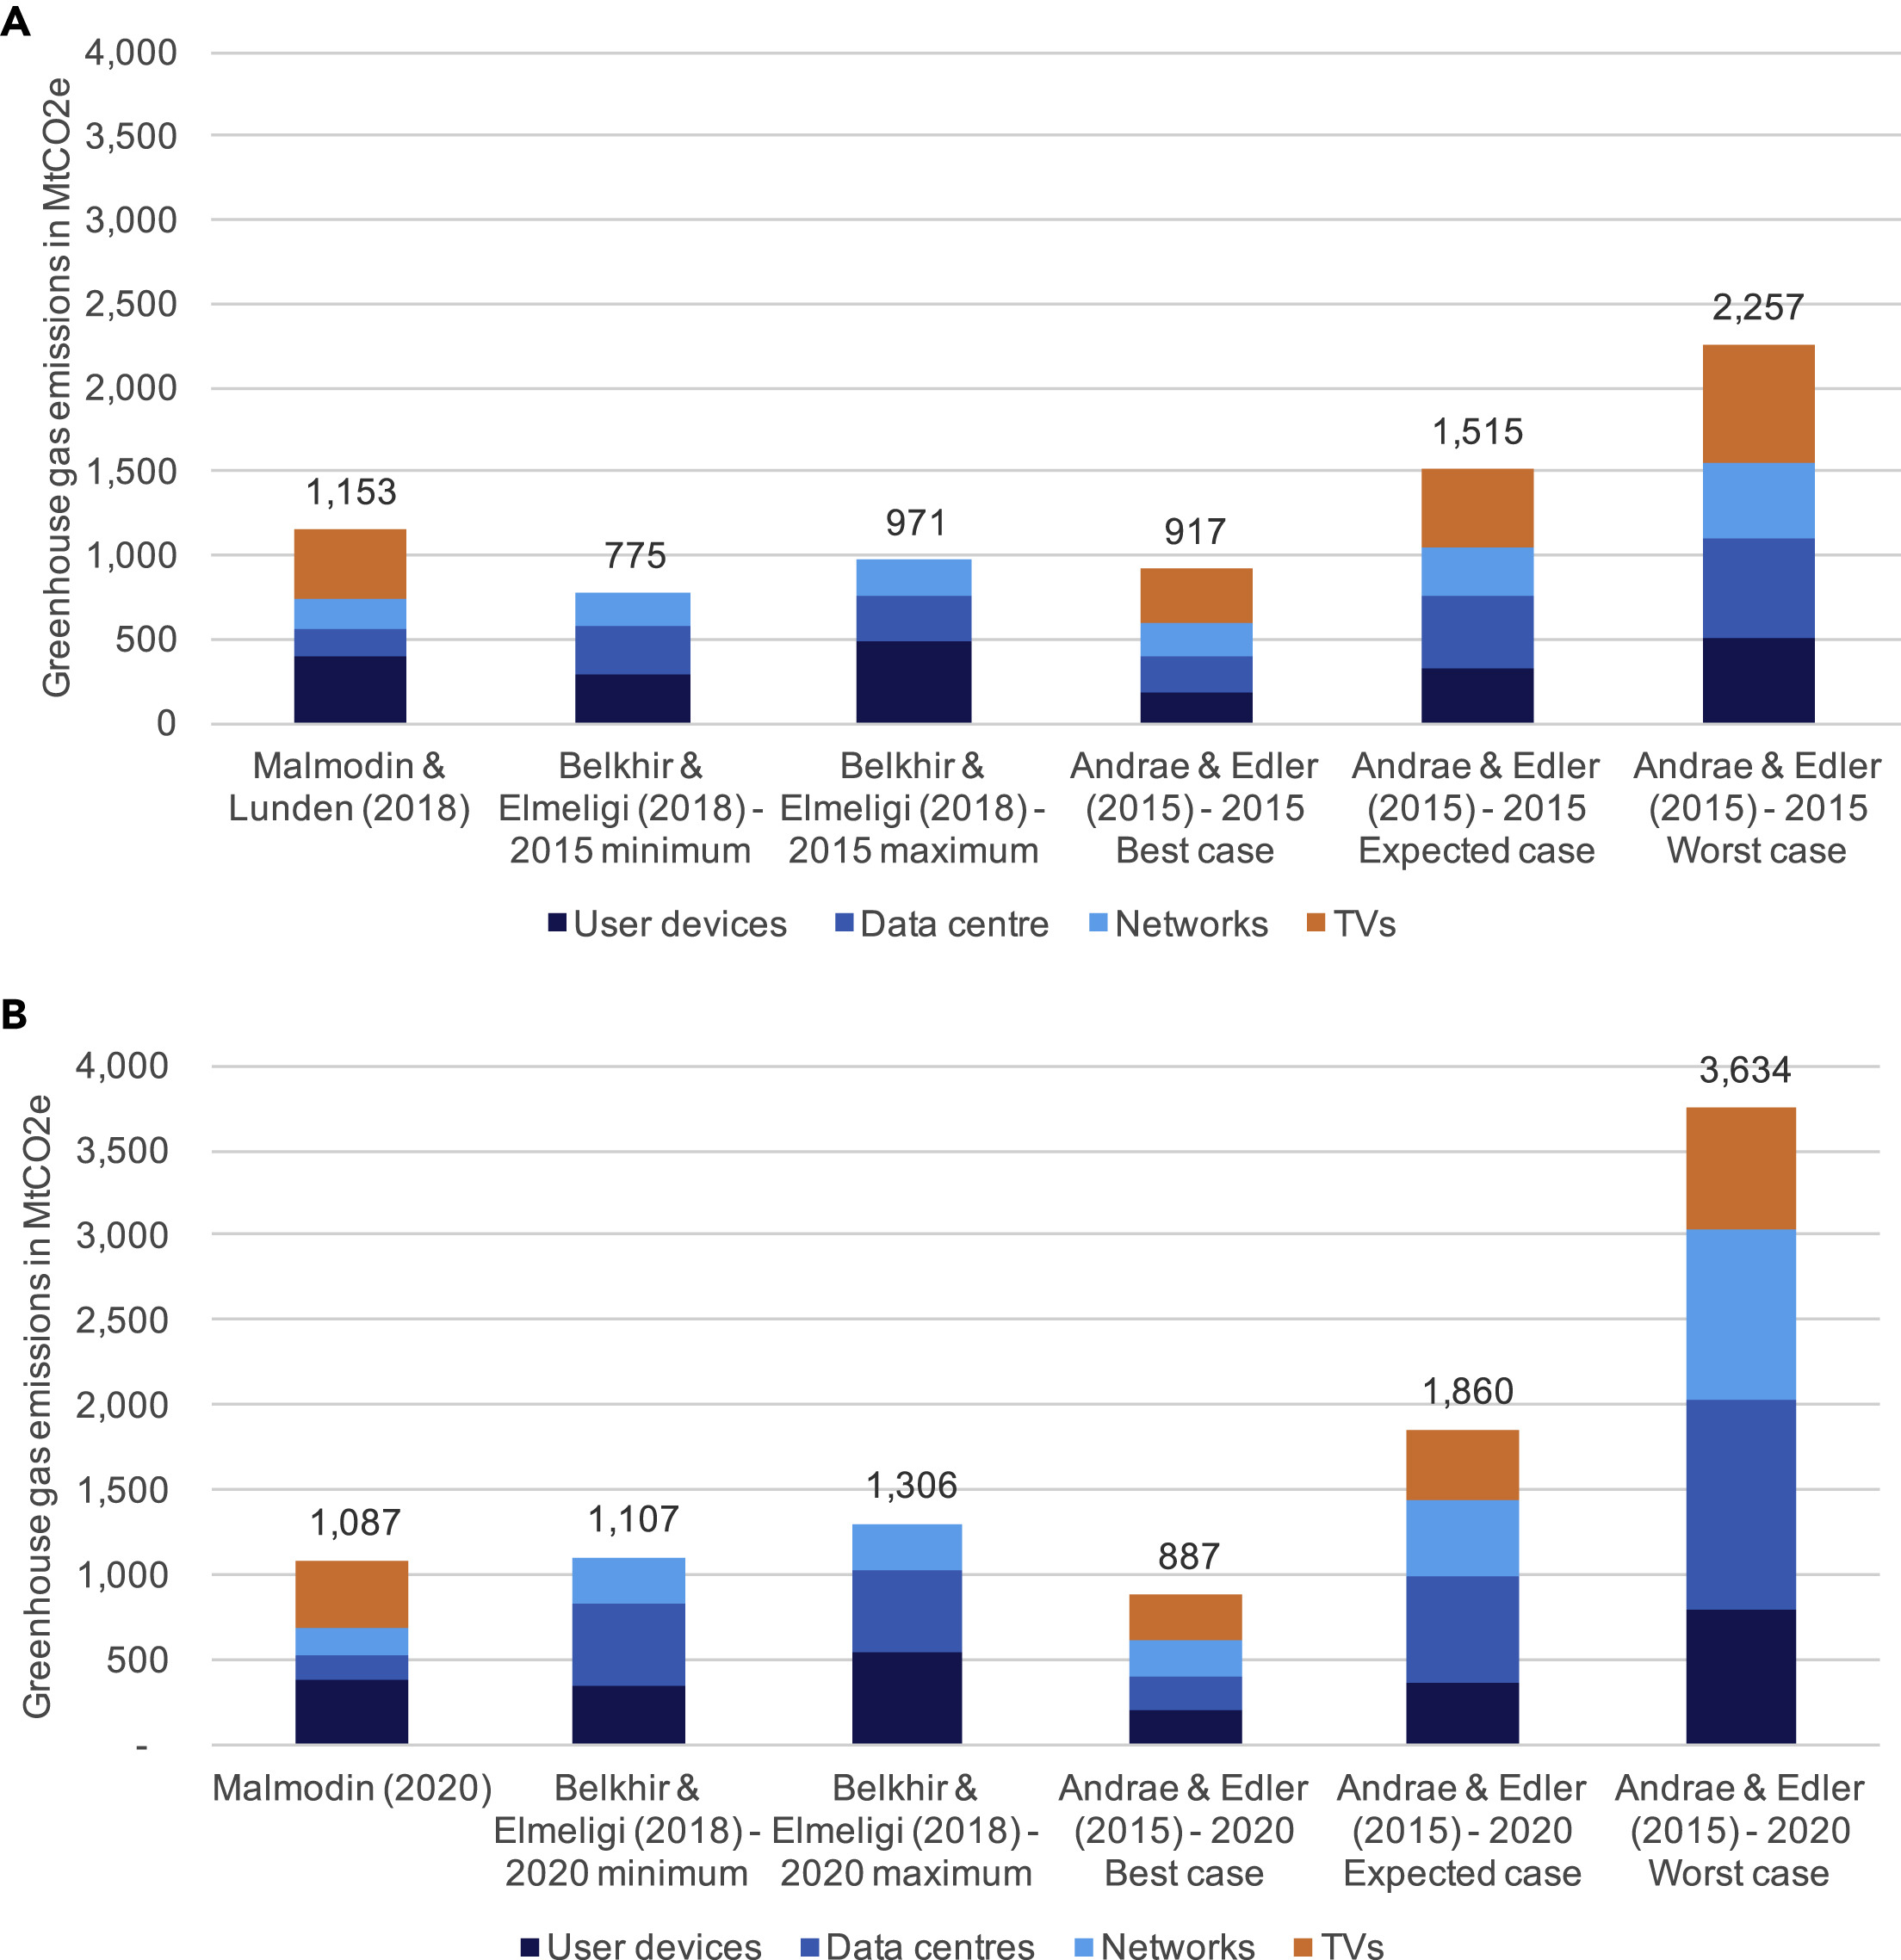
\includegraphics[scale=0.8]{Images/Related_works/gr2_lrg.jpg}
%     \caption[Estimations for global ICT’s GHG emissions in 2015 and 2020]{Estimations for global ICT’s GHG emissions in 2015 and 2020 \cite{freitag2021climate}. The authors consolidated the works from \cite{belkhir2018assessing, andrae2015global, malmodin2018energy, Malmodin2020}.}
%     \label{fig:estimations_ICT}
% \end{figure}

Data centers are very energy consumers. IEA published an article indicating that data centers and networks were responsible for almost 1\% of energy-related GHG emissions in 2020 \cite{centres2022data}. Google data centers consumed the same amount of energy as the entire city of San Francisco in 2015 \cite{khan2018exploiting}. Global data center electricity usage in 2021 was 220-320 TWh, corresponding to 0.9-1.3\% of the global demand \cite{centres2022data}. For example, the domestic electricity consumption of Italy was 300 TWh in 2021 \cite{ElectricityDomesticConsumption}. In Ireland, electricity consumed by data centers went from 5\% of the total electricity consumption in 2015 to 14\% in 2021 \cite{IrelandDatacenter}. Denmark predicts tripling data center consumption, corresponding to 7\% of the country’s electricity use \cite{DenmarkDatacenter}.

Despite the strong growth in demand, data center energy usage has only moderately grown \cite{centres2022data}. A reason that explains it is the improvements in IT energy consumption (in hardware and software). These improvements allowed a boost in microchips' speed with a reduction in their power consumption, letting big data center companies cope with the peak in demand. Gordon Moore predicted in 1965 (Moore's law) that \cite{moore1965cramming}:

\begin{quote}
    ``The complexity for minimum component costs has increased at a rate of roughly a factor of two per year. Certainly over the short term this rate can be expected to continue, if not to increase. Over the longer term, the rate of increase is a bit more uncertain, although there is no reason to believe it will not remain nearly constant for at least 10 years.''
\end{quote}

Even if he predicted it just until 1975, it is the case nowadays. However, the future is uncertain, and the community is divided to confirm continuous efficiency improvements \cite{freitag2021climate}. While Andrae and Edler \cite{andrae2015global} and Belkhir and Elmeligi \cite{belkhir2018assessing} expected an ending in power-consuming improvements (indicated in Figure \ref{fig:projections_ICT}), Malmodin and Lundén \cite{malmodin2018energy} are more optimistic. They suggest that ICT’s carbon footprint in 2020 could halve by 2030. To achieve that, he considers two key factors. First, the improvements will continue. However, all these improvements are not enough because of the increase in usage (demonstrated in Figure \ref{fig:projections_ICT}). Second, the migration to renewable sources.

% \begin{itemize}
%     \item Present the numbers of global warming generally;
%     \item Present the predictions about the global warming;
%     \item Introduce the role of ICT generally;
%     \item Write about data center impact;
% \end{itemize}

\section{Renewable Energy Sources}

The ICT migration to renewable energy sources (RES) is one of the factors that helped reduce the growth in GHG emissions despite the rapidly growing demand for digital services \cite{centres2022data}. RES is one of the principal solutions to decarbonize electrical production \cite{olabi2022renewable, rostirolla2022survey}. RES is also named green energy, in contrast to brown energy from fossil fuels. Basically, RES generates energy from natural sources, such as solar, wind, geothermal, hydropower, wave and tidal, and biomass \cite{augustine2012renewable, panwar2011role, rostirolla2022survey, UNREnewable, gross2003progress}. These natural sources have a low impact on GHG emissions. For example, manufacturing is the stage with higher emissions for wind and solar \cite{amponsah2014greenhouse}. So, these components could produce energy with no or low GHG emissions. The renewable term comes from the idea that these sources are constantly replenished. On the other hand, fossil fuels are non-renewable because they need hundreds of millions of years to develop. In the Net Zero Emissions by 2050 Scenario, RES is responsible for one-third of the reductions between 2020 and 2030 \cite{renewables2022}. Some countries focus on nuclear power plants to produce energy. Even if nuclear power is a low carbon emissions energy source, it introduces the risk of accidents and environmental impacts of radioactive wastes \cite{kunsch2014nuclear}. It also consumes a lot of water.

The biggest challenge of implementing RES is its intermittence \cite{rostirolla2022survey}. Since RES production comes from nature, it depends on the climate conditions. For example, there is no power production from solar during the night. There are two approaches for implementing RES production: on-site and off-site generation \cite{ren2012carbon}. On-site generation uses local renewable resources, and off-site takes resources available on the grid. In an off-site generation, it is not possible to guarantee that the incoming energy is from RES since the grid mixes all types of power generation \cite{rostirolla2022survey}. Giant cloud providers (e.g., Google, Amazon, and Facebook) invest in solar and wind power plants in an off-site approach \cite{Masanet984, branscombe2020google, amazon2023}. So, they could say that they provide RES to the grid with the same amount that they expend. However, they transfer the RES uncertainty problem to third parties \cite{rostirolla2022survey}. For example, in a case with a peak in demand, they will use the power from the grid, renewable or not. Therefore, they are still non-renewable-dependent.

\section{Renewable-only Data center}
Since data centers have a stable infrastructure (e.g., the number of servers tends to stay constant, the network is stable, changes in the infrastructure are planned, etc.), they are a good target to migrate to a renewable-only environment \cite{rostirolla2022survey}. However, creating a renewable-only data center imposes several challenges. In a data center using grid energy, a manager receives the tasks from the users and defines a placement. This manager focuses on maintaining a good QoS. However, in a renewable-only data center, the manager also needs to control the available energy usage. In this kind of data center, all the generation is on-site without backup from the grid. Nevertheless, the production and demand can not match. Figure \ref{fig:load_production} exemplifies the mismatch between the power demanded by a data center and power generation. This mismatch requires a production (electrical) or a load (IT) shift. This thesis focuses on the manager in a renewable-only data center. We will present both electrical and IT elements needed for this kind of data center.

\begin{figure}[!htb]
    \centering
    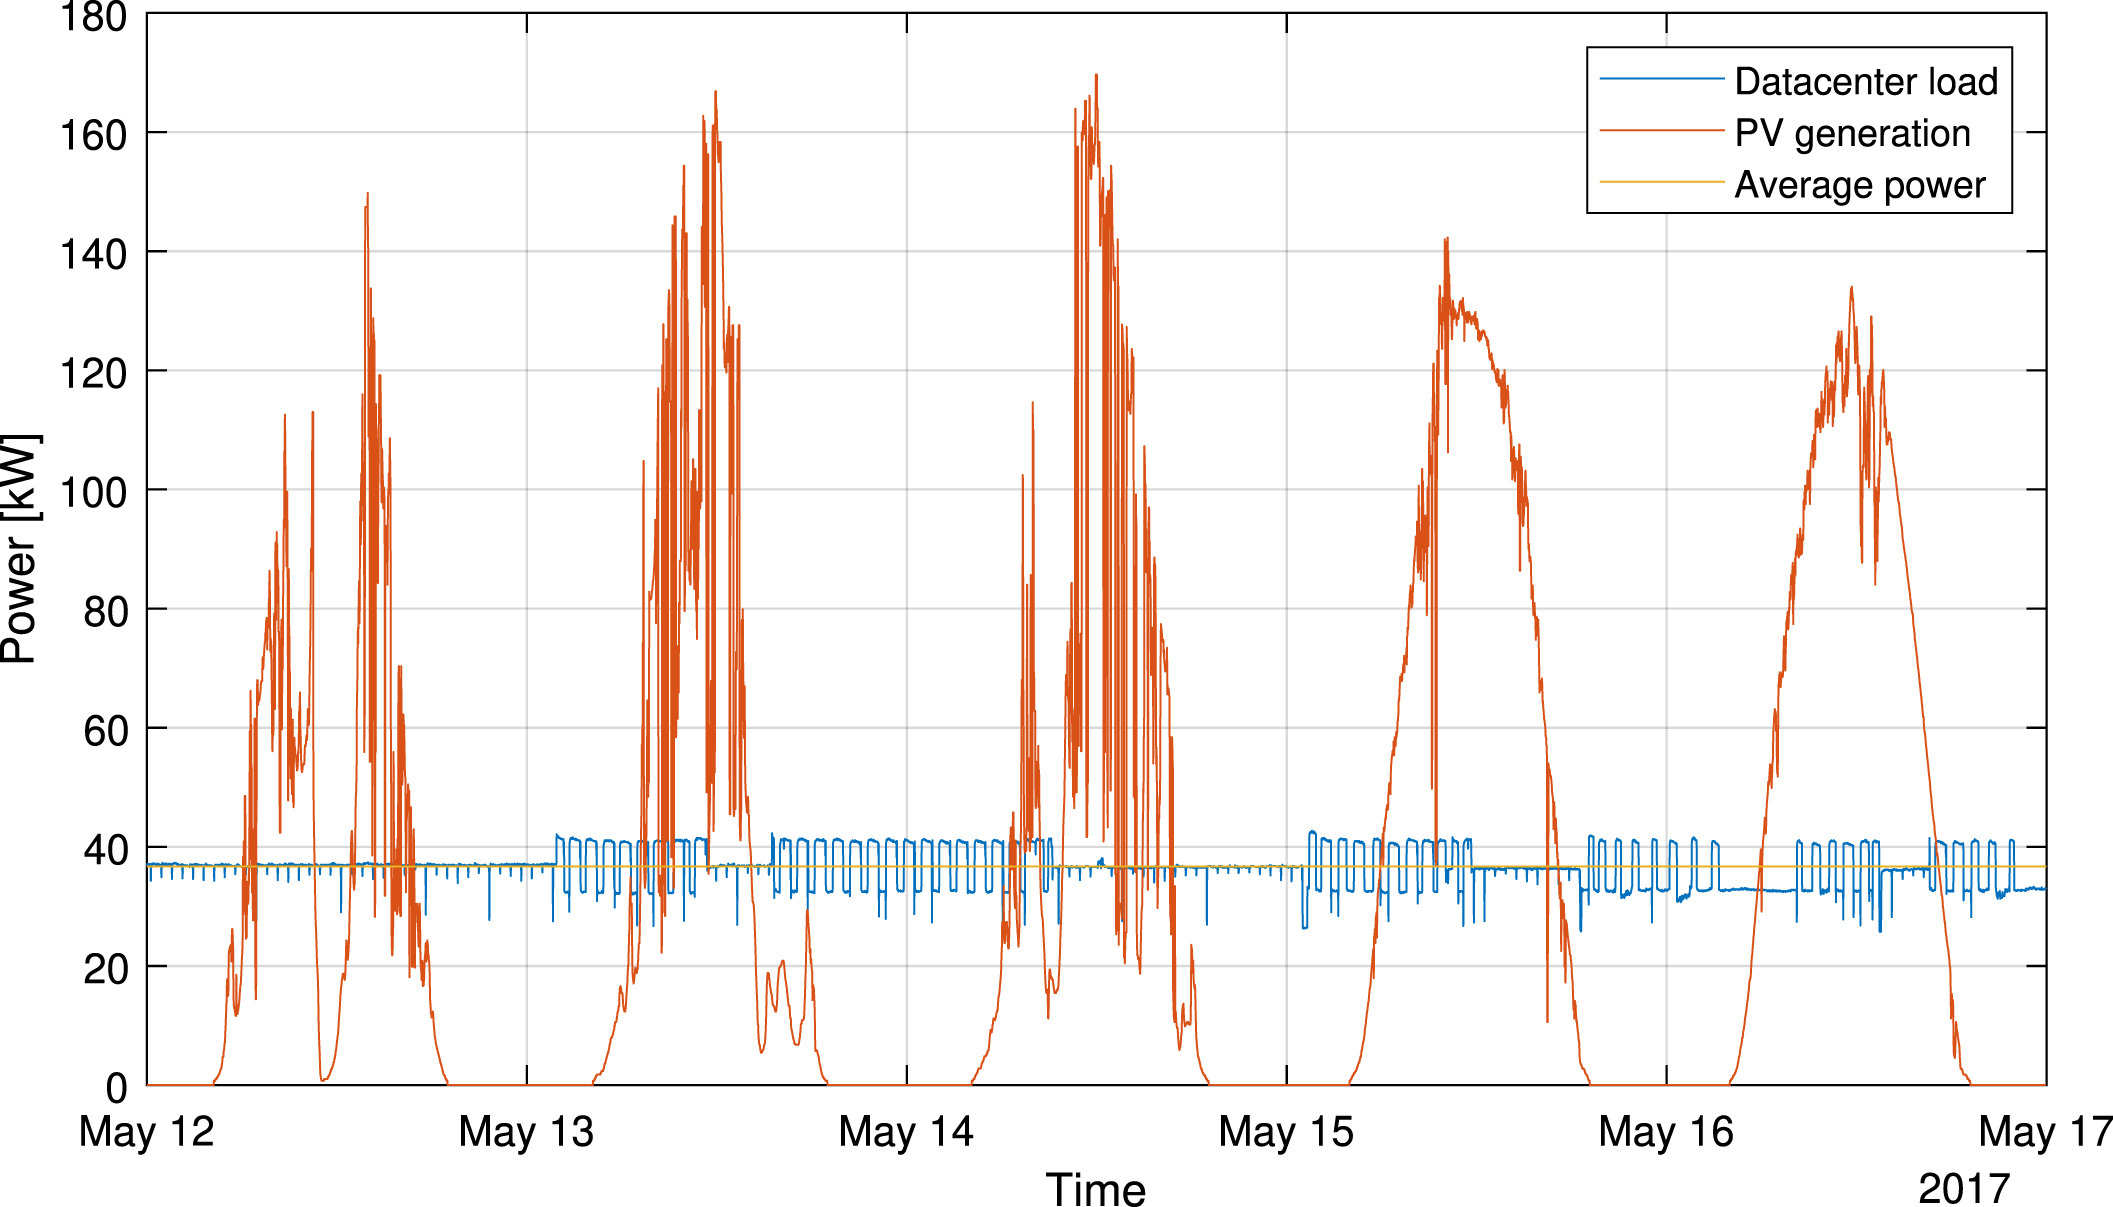
\includegraphics[scale=1]{Images/Related_works/load_production.jpg}
    \caption[Comparison of small data center load and the generation from a theoretical photovoltaic in Belfort, France. Both load and production have the same average value.]{Comparison of small data center load and the generation from a theoretical photovoltaic in Belfort, France. Both load and production have the same average value \cite{rostirolla2022survey}.}
    \label{fig:load_production}
\end{figure}

% \begin{itemize}
%     \item Explain the possibility of applying renewable in data centers;
%     \item Present the challenges in a renewable-only data center;
% \end{itemize}

\subsection{Electrical elements}
\label{sec:related_work_electrical_elements}
As mentioned before, different renewable sources can generate power. We focus on wind and solar since they are the most prominent in current years \cite{renewables2022}. For wind turbines, the wind speed is crucial. Equation \ref{equ:wind_turbines} gives the power output $P_{wt}(t)$ at the moment $t$ of a wind turbine, given the wind speed $v$ \cite{garcia2006wind, dong2016optimal, maleki2015optimal}.

\begin{equation}
    \label{equ:wind_turbines}
    P_{wt}(t) = \begin{cases}
        0 & v \leq v_{in} \text{ or } v(t) > v_{out} \\
        P_{WT,rated} \times \frac{v(t) - v_{in}}{v_{rated} - v_{in}} & v_{in} < v(t) \leq v_{rated} \\
        P_{WT,rated} & v_{rated} < v(t) \leq v_{out}
    \end{cases}
\end{equation}

Where:
\begin{itemize}
    \item $P_{wt}(t)$: Power generated by a wind turbine (kW);
    \item $v$: Wind speed (m/s);
    \item $v_{in}$: Cut-in wind speed (m/s);
    \item $v_{out}$: Cut-out wind speed (m/s);
    \item $v_{rated}$: Speed related to wind turbine nominal power (m/s);
    \item $P_{WT,rated}$: Wind turbine nominal power (kW).
\end{itemize}

If the wind speed $v$ is lesser or equal to the cut-in $v_{in}$  or greater than the cut-out $v_{out}$, it does not produce power. It tests the cut-out $v_{out}$ to protect the generator. If the speed $v$ is greater than the cut-in $v_{in}$ and lesser or equal to the rated speed $v_{rated}$, it generates proportionally to the rated power $P_{WT,rated}$ and rated speed $v_{rated}$. Finally, if the speed $v$ is greater than the rated speed $v_{rated}$ and lesser or equal to the cut-out $v_{out}$, it produces constant power $P_{WT,rated}$. 

Regarding solar production, the photovoltaic (PV) system uses solar panels to generate power from solar irradiance. Equation \ref{equ:panel_solar_with_temperature} demonstrates how to calculate the output power of a solar panel $P_{pv}(t)$ \cite{maleki2015optimal, sinha2015review, dong2016optimal}.

\begin{equation}
    \label{equ:panel_solar_with_temperature}
    P_{pv}(t) = P_{R,PV} \times (R / R_{ref}) \times \eta_{PV}
\end{equation}

Where:
\begin{itemize}
    \item $P_{pv}(t)$: Power generated by each PV panel (W);
    \item $P_{R,PV}$: PV panel Nominal power (kW);
    \item $R$: Solar irradiance (W/$m^{2}$);
    \item $R_{ref}$: solar irradiance at reference conditions. Usually set as 1000 (W/$m^{2}$) \cite{dong2016optimal};
    \item $\eta_{PV}$: PV efficiency, including power eletronics and power point control \cite{sinha2015review, maleki2015optimal}.
\end{itemize}

% Regarding PV efficiency $\eta_{PV}$, it can consider the temperature of the solar panel \cite{sinha2015review, maleki2015optimal}. 
Some works simplify PV efficiency by applying a constant value \cite{dong2016optimal, haddad2019mixed}. Equations \ref{equ:wind_turbines} and \ref{equ:panel_solar_with_temperature} demonstrate that both wind turbines and solar panels depend on wind speed and solar irradiance, respectively. So, the weather conditions drive how much power both can generate. 

Due to the weather intermittence, it is necessary to introduce storage elements. These storage elements allow for shifting generation and consumption over time \cite{rostirolla2022survey}. For example, power coming from wind turbines during the night can be stored and used during the day. Big companies are investing in massive storage elements. An example is Google which is planning a 350 MW solar plant in Nevada connected to a storage system with a maximal power of 280 MW \cite{branscombe2020google}. There are different types of storage with advantages and drawbacks \cite{wang2012energy}. One of them is hydropower and underground compressed air storage. However, this kind of storage is very geographical, geological, and terrain dependent, which makes it inappropriate to use in data centers \cite{rostirolla2022survey}. Another type is the very short-term storage such as flywheels or supercapacitors. These storages can output and absorb energy over ms to minutes \cite{wang2012energy}. They are very suitable for maintaining power stability but not for storing energy for a larger time horizon (e.g., hours or days) \cite{rostirolla2022survey}. In this thesis, we focus on the batteries and Hydrogen Storage System (HSS).

Batteries are electrochemical devices that store energy in chemical form \cite{rostirolla2022survey, yilanci2009review, wang2012energy}. They are very reactive because they do not need a warm-up to store/generate power. Batteries are good for short-term storage scenarios (e.g., several hours, day/night cycles) \cite{rostirolla2022survey}. However, they are inappropriate for longer periods due to their self-discharge rate and low energy density \cite{rostirolla2022survey, yilanci2009review}. Historically, Uninterruptible Power Supply (UPS) added batteries to avoid the server's blackout, doing a soft shutdown that avoids several problems, such as data loss, data corruption, work loss, etc. A problem with batteries is the degradation in capacity and performance over time, requiring battery replacement \cite{rostirolla2022survey}. A way to extend battery life is by avoiding charging/discharging too extensively \cite{xu2016modeling}. There are some methods to model the energy level inside the battery, such as energy-based, Current-based, or State of Charge \cite{rostirolla2022survey}. We focus on the State of Charge since it represents the percentage of energy inside the battery according to its capacity (e.g., 100\% means battery full and 0\% dry). \citeauthor{xu2016modeling} present results showing that maintaining SoC at a narrow range reduces battery degradation \cite{xu2016modeling}. However, using a narrow range would reduce the battery's effectiveness because it can deliver less energy to deal with intermittence. So, the battery SoC must be maintained within a range considering this trade-off. Equations \ref{equ:battery_energy} and \ref{equ:battery_state_of_charge} demonstrate how to calculate the State of Charge \cite{haddad2019mixed}. 

\begin{equation}
    \label{equ:battery_energy}
    E_{bat}(t) = (E_{bat}(t-1) \times (1 - \sigma)) + (P_{ch}(t-1) \times \eta_{ch} \times \Delta t) - (P_{dch}(t-1) \times \eta_{dch} \times \Delta t)
\end{equation}
\begin{equation}
    \label{equ:battery_state_of_charge}
    SoC(t) = \frac{E_{bat}(t)}{C_{bat}} \times 100
\end{equation}

Where:
\begin{itemize}
    \item $\Delta t$: Duration of $t$ (h);
    \item $E_{bat}(t)$: Energy in the battery at instant $t$ (kWh);
    \item $P_{ch}(t)$: Charging power (kW);
    \item $P_{dch}(t)$: Discharging power (kW);
    \item $\sigma$: Battery self-discharge rate (\%);
    \item $\eta_{ch}$: Battery charge efficiency (\%);
    \item $\eta_{dch}$: Battery discharge efficiency (\%);
    \item $C_{bat}$: Capacity of the battery (kWh);
    \item $SoC(t)$: State of Charge at instant $t$ (\%);
\end{itemize}

We can divide Equation \ref{equ:battery_energy} into three parts. The first part ($E_{bat}(t-1) \times (1 - \sigma)$) calculates the natural self-discharge, ignoring charging or discharging the battery. The second part ($P_{ch}(t-1) \times \eta_{ch} \times \Delta t$) computes the energy stored in the battery according to the charging power. The last part ($P_{dch}(t-1) \times \eta_{dch} \times \Delta t$) is similar but for discharging. Both charging and discharging are not perfect with some losses given by $\eta_{ch}$ and $\eta_{dch}$. For example, if we apply 1 kW this does not mean that, after one hour, we charged 1 kWh. We will charge $1 kW \times \eta_{ch}$ (where $\eta_{ch} < 1$). Besides, we can not charge and discharge the battery simultaneously, so if $P_{ch} > 0$ then $P_{dch} = 0$, and vice-versa \cite{haddad2019mixed}. Equation \ref{equ:battery_state_of_charge} normalizes the SoC to percentage.

Hydrogen, likely the batteries, is a reversible energy storage, allowing to charge and discharge. However, it is more suitable for long-term storage (e.g., over seasons), mainly because it can store large amounts of energy with very low self-discharge \cite{pregger2009prospects}. A big limitation of this kind of storage is the lack of reactivity since it demands a longer warming-up time. Furthermore, it includes performance degradation concerns, low efficiency compared to batteries, high costs, and complicated safety measures \cite{rostirolla2022survey}. Even with all these drawbacks, it is a good solution for storing energy during abundant periods (e.g., summer) and using it during lacking periods (e.g., winter). Three elements compose an HSS: electrolyzer, hydrogen tank, and fuel cell. The electrolyzer produces hydrogen from electricity, according to Equation \ref{equ:hydrogen_electrolyzer} \cite{haddad2019mixed}.

\begin{equation}
    \label{equ:hydrogen_electrolyzer}
    E_{ez} = P_{ez}(t) \times \Delta t = \frac{HH_{h_{2}} \times Q_{ez}(t)}{\eta_{ez}}
\end{equation}

Where:
\begin{itemize}
    \item $\Delta t$: Duration of $t$ (h);
    \item $E_{ez}$: Energy put into the electrolyzer ($P_{ez}(t) \times \Delta t$);
    \item $P_{ez}(t)$: Power put into electrolyzer (kW);
    \item $HH_{h_{2}}$: $H_2$ higher heating value ($kWh / kg$);
    \item $Q_{ez}(t)$: Electrolyzer $H_2$ mass flow (kg);
    \item $\eta_{ez}$: Electrolyzer efficiency (\%).
\end{itemize}

This equation indicates how much hydrogen is added to the tank ($Q_{ez}(t)$) according to the electrolyzer operating power ($P_{ez}(t)$). On the other hand, the fuel cell transforms hydrogen into electricity, according to Equation \ref{equ:hydrogen_fuel_cell} \cite{haddad2019mixed}.

\begin{equation}
    \label{equ:hydrogen_fuel_cell}
    E_{fc} = P_{fc}(t) \times \Delta t = LH_{h_{2}} \times Q_{fc}(t) \times \eta_{fc}
\end{equation}

Where:
\begin{itemize}
    \item $\Delta t$: Duration of $t$ (h);
    \item $E_{fc}$: Energy delivered by fuel cell ($P_{fc}(t) \times \Delta t$);
    \item $P_{fc}(t)$: Power delivered by fuel cell (kW);
    \item $LH_{h_{2}}$: $H_2$ lower heating value ($kWh / kg$);
    \item $Q_{fc}(t)$: Fuel cell $H_2$ mass flow (kg);
    \item $\eta_{fc}$: Fuel Cell efficiency (\%).
\end{itemize}

Similarly, this equation indicates how much hydrogen is removed from the tank ($Q_{fc}(t)$) according to the output power of the fuel cell ($P_{fc}(t)$). To calculate the Level of Hydrogen ($LoH(t)$ (kg)) Equation \ref{equ:hydrogen_level}, consolidates the result of the electrolyzer and the fuel cell.

\begin{equation}
    \label{equ:hydrogen_level}
    LoH(t) = LoH(t-1) + Q_{ez}(t-1) - Q_{fc}(t-1)
\end{equation}

\subsection{IT elements}
\label{sec:related_work_it_elements}
While electrical elements are power producers (wind turbines and solar panels) or producers/consumers (batteries and hydrogen), the IT elements are entirely power consumers. IT power consumption can be divided into two parts: IT hardware (e.g., servers, data storage, and network devices) and supporting infrastructure (e.g., cooling equipment) \cite{centres2022data, dayarathna2015data}. This thesis focus on computing nodes (servers) and scheduling policies on the IT side, so we do not consider data storage, network devices, and supporting infrastructure. There are several articles dealing specifically with these components \cite{dayarathna2015data, orgerie2014survey, zhang2021survey, hammadi2014survey, yuan2022optimal}. The servers are powerful, high-performance machines designed to handle intensive computational tasks and ensure the efficient functioning of various applications and services. They are optimized for reliability, scalability, and performance. Even with these optimizations, they do not have a negligible power consumption \cite{ismail2020computing, orgerie2014survey}.

The server power consumption is divided into two parts: static and dynamic \cite{orgerie2014survey, heinrich2017predicting}. Static power consumption is constant and given by current leakage present in any powered system. Dynamic power is not constant and depends on computing usage. There are different models to estimate power consumption, such as mathematical linear and non-linear, linear regression, lasso regression, support vector machines, etc \cite{ismail2020computing}. Equation \ref{equ:cpu_usage} expresses a mathematical linear representation of static and dynamic power \cite{heinrich2017predicting, ismail2020computing}.

\begin{equation}
    \label{equ:cpu_usage}
    Pcpu(t) = P^{static} + (P^{dynamic} \times u_{cpu})
\end{equation}

Where:
\begin{itemize}
    \item $Pcpu(t)$: Power consumption at moment $t$ (W);
    \item $P^{static}$: Static power consumption (W);
    \item $P^{dynamic}$: Dynamic power consumption (W);
    \item $u_{cpu}$: CPU usage (\%);
\end{itemize}


While \citeauthor{ismail2020computing} indicate that $P^{static}$ can be considered as the power idle \cite{ismail2020computing}, \citeauthor{heinrich2017predicting} demonstrate a slight difference between the power usage at fully idle and when the real $P^{static}$ \cite{heinrich2017predicting}. Power idle (or $P_{idle}$ in Figure \ref{fig:cpu_frequency_consumption}) is the CPU power usage when all its cores are idle with nothing running. The processor enters a power-saving mode, reducing power consumption. On the other hand, $P^{static}$ is the power consumption when at least one core is running something. Then, starting with $P^{static}$, the relation between the number of active cores and power is linear, as presented in Figure \ref{fig:cpu_frequency_consumption}. The work of \citeauthor{heinrich2017predicting} is the base for a well-known data center simulator named Simgrid\footnote{https://simgrid.org/} and its evolutions. This article also indicates that $P^{dynamic}$ depends on the application and the server frequency. Figure \ref{fig:cpu_frequency_consumption} shows the linearization of the power consumption according to the frequency for the same application. Setting different frequencies is possible through the Dynamic Voltage and Frequency Scaling (DVFS) technique. Putting the server at a lower frequency reduces the server's power consumption (as illustrated in Figure \ref{fig:cpu_frequency_consumption}). However, it also decreases the server's speed. Nevertheless, DVFS is a possible solution to reducing energy consumption in moments with lower power available. 

\begin{figure}[!htb]
    \centering
    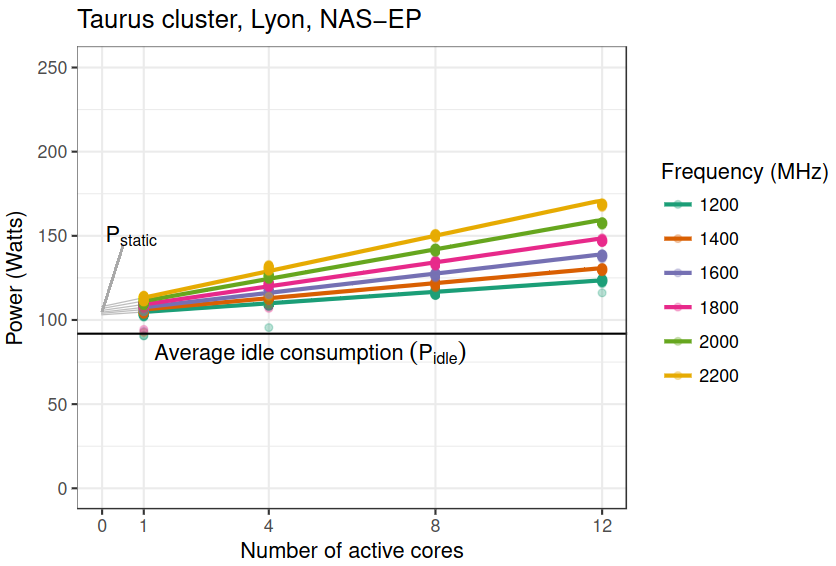
\includegraphics[scale=0.4]{Images/Related_works/cpu_usage.png}
    \caption[Power consumption on a GRID5000 server when running the same application, but varying the frequency and the number of active cores.]{Power consumption on a GRID5000 server when running the same application, but varying the frequency and the number of active cores \cite{heinrich2017predicting}.}
    \label{fig:cpu_frequency_consumption}
\end{figure}

Another possibility, more drastic, is putting the server to sleep. In the sleep state, the server is unavailable but consuming the lowest possible. Besides being inaccessible, another consideration in the sleep state is that sleep transitions (on$\rightarrow$off and off$\rightarrow$on) are not instantaneous and waste energy. \citeauthor{rais2018quantifying} present a Dynamic Power Management (DPM) solution \cite{rais2018quantifying}. This DPM estimates a $T_{wait}$ threshold that when the server is idle for more than $T_{wait}$ seconds, it is more energy-efficient to switch the server off. Equation \ref{equ:dpm_waiting_time} represents their idea.

\begin{equation}
    \label{equ:dpm_waiting_time}
    T_{wait} = \max(\frac{E_{OnOff} + E_{OffOn} - (P_{Off} \times (T_{OnOff} + T_{OffOn}))}{P_{idle} - P_{Off}}, (T_{OnOff} + T_{OffOn}))
\end{equation}

Where:
\begin{itemize}
    \item $T_{wait}$: Waiting time before putting the server to sleep (s);
    \item $P_{idle}$: Power consumption when the server is unused, but powered on (W);
    \item $P_{Off}$: Power consumption when the server is off (not null and lower than $P_{idle}$) (W);
    \item $E_{OnOff}$: Energy consumed during the On$\rightarrow$Off transition (J);
    \item $E_{OffOn}$: Energy consumed during the Off$\rightarrow$On transition (J);
    \item $T_{OnOff}$: Time spent by the server on On$\rightarrow$Off (s);
    \item $T_{OffOn}$: Time spent by the server on Off$\rightarrow$On (s);
\end{itemize}

A data center's main objective is to execute users' applications. Running applications in the servers variates the server's CPU usage $u_{cpu}$. Data centers receive plenty of different application types. We can separate these applications into two big categories: services and batch \cite{rostirolla2022survey,da2018modeling}. Services are applications that interact with different clients. These clients make requests answered by a running service. Each request has a low processing time, but the ensemble of these requests can be very CPU-consuming \cite{masdari2020survey}. In addition, the service must answer the request as soon as it arrives. On the other hand, batch applications (or parallel jobs \cite{feitelson2014experience}) do not run interactively. While services can run indefinitely, batches have a start and end time. Usually, these applications aim to solve complex problems, such as weather prediction, optimization problems, and simulations, being very long and CPU-consuming \cite{masdari2020survey}. Batch jobs are more flexible considering the moment to execute them, allowing the batch scheduler to define the best moment in the future to run them. Both services and batches demand different approaches and algorithms to deal with them. This thesis focuses on batch applications. An batch job is composed by \cite{rostirolla2022survey, srinivasan2002characterization, takizawa2020effect}:

\begin{itemize}
    \item \textit{Submission time}: The moment when the user sends the job;
    \item \textit{Requested resources}: The resources demanded by the job, such as the number of cores, servers, memory, etc;
    \item \textit{Estimated execution time or walltime}: The user indicates how long the job executes. If the real execution time is equal to the walltime, the scheduler kills the job. 
\end{itemize}

One of the most important components in a data center is the scheduler. The scheduler is responsible for managing all the IT elements. The scheduler actions are:
\begin{itemize}
    \item \textit{Job filtering}: The scheduler must accept or reject incoming jobs from users. For example, it can reject a job because it is too big to process in this data center;
    \item \textit{Waiting queue management}: All the accepted jobs wait in a queue. The scheduler uses this list to take the jobs to process. Additionally, the scheduler can sort the list by any metric, such as size, importance, arrival (e.g., First-Come, First-Served), etc.;
    \item \textit{Job placement}: The scheduler selects a server to process a job from the waiting queue. The server must match the job's resource requirements (e.g., memory, processors, storage, etc.);
    \item \textit{Execution management}: The scheduler can capture metrics of the execution of the jobs, such as execution time, energy usage, CPU usage, job state, etc. These metrics can help in decision-making. It can interrupt the job execution, killing, suspending (to finish later), or migrating it. In addition, it should kill the jobs with execution time higher than the walltime given by the user, avoiding a job with infinity execution using the resources;
    \item \textit{Server configuration}: In a power-aware system such renewable-only data center, the scheduler must set the server's states. The server state can be sleeping or running at some speed (through DVFS). So, it can turn on servers to deal with new jobs or shutdown or change the processor's frequency to save energy;
\end{itemize}
All these responsibilities make the scheduler a crucial element of optimization in a data center. It is even more important with the introduction of renewable-only power constraints.

% \begin{itemize}
%     \item Write about the servers;
%     \item Write about the power consumption (e.g., DVFS, on-off, idle, etc);
%     \item Write about the jobs (e.g., types, resources demanded, etc);
% \end{itemize}

\section{Sources of Uncertainty}

After describing renewable-only data center elements, in this section, we detail the sources of uncertainty. First, we start presenting the uncertainty from electrical components due to weather conditions. After that, we describe the uncertainties from server power consumption and batch jobs. Finally, we discuss the challenges in dealing with all these uncertainties.

\subsection{Weather Uncertainties}
\label{sec:weather_uncertainties}

As presented in Section \ref{sec:related_work_electrical_elements}, the objective of the electrical components (solar panels and wind turbines) is to generate power. So, they transform natural renewable resources into energy. Due to the intermittence of these renewable resources, the output power is also intermittent \cite{perez2011managing}. Regarding solar panels, the output power is calculated easily, using Equation \ref{equ:panel_solar_with_temperature}, in a "clear-sky" condition \cite{tuohy2015solar}. "Clear-sky" considers an exposition total of the panels to the sun. However, solar irradiance is impacted by several weather conditions, such as clouds, aerosols, and other atmospheric constituents \cite{tuohy2015solar}. Besides, the panel efficiency is temperature dependent. Concerning wind turbines, the power output depends on the wind speed (see Equation \ref{equ:wind_turbines}). The production has lower and higher wind speed thresholds, meaning that even too slow/fast wind will not produce power. 

Due to the renewable intermittence, it is crucial to forecast weather conditions to estimate future power production. Several works propose ways to predict these conditions \cite{tuohy2015solar, soman2010review, sharma2018review, ssekulima2016wind}. Two key terms are important in renewable production: Predictability and Variability \cite{ssekulima2016wind, perez2011managing}. Predictability means the ability to anticipate the availability of a generation resource \cite{perez2011managing}. For example, solar irradiance is more predictable than wind speed because the forecast accuracy on clear days is high, and satellite data tracks precisely the direction and speed of clouds \cite{perez2011managing}. On the other hand, due to the erratic nature of the atmosphere, there is randomness in wind power production \cite{sharma2018review}. Variability indicates the variation over time in production \cite{perez2011managing}. Both wind and solar can vary. For example, the wind has high variability because it will deviate from 0\%–100\% over a day \cite{perez2011managing}. Another element that influences forecast accuracy is the time horizon. For example, the next five minutes are more predictable than the next three days.

Besides the weather conditions, the material can also introduce uncertainties. Two elements (wind turbines and solar panels) of the same model can produce energy differently. Besides, different battery cells and hydrogen components have different efficiency. Another aspect is the impact of aging on the elements efficiently. Furthermore, these elements can have failures, reducing the total power production. Therefore, it is hard to model the exact electrical elements' power production, charge, and discharge. 

% \begin{itemize}
%     \item Describe wind uncertainty;
%     \item Describe solar irradiance uncertainty;
% \end{itemize}

\subsection{Server Uncertainties}
Estimating the real power consumption of a server is not trivial. Several works try to find a model to describe energy consumption or even apply machine learning to define it \cite{dayarathna2015data}. Even two machines with the same configuration can consume differently \cite{orgerie2010demystifying}. It is also true that distinct applications can have completely different energy consumption, mainly because they use the CPU differently \cite{orgerie2010demystifying, jay2023experimental}. Equation \ref{equ:cpu_usage} presents a simplification of server power consumption. However, this equation is still applicable since different servers can have different dynamic ($P^{dynamic}$) and static ($P^{static}$) power. Considering that energy consumption is the integral of Equation \ref{equ:cpu_usage}, different applications can have distinct CPU usage ($u_{cpu}$) over time. Even if the equation is still appropriate, predicting its parameters is challenging. For example, the CPU usage ($u_{cpu}$) of a job can vary between executions (e.g., due to different application parameters). Furthermore, new applications do not have records to estimate their usage. Considering the static power ($P^{static}$), it is known that it can vary according to the processor's heat \cite{patterson2008effect}.

\subsection{Workload Uncertainties}
Besides impacting server consumption, jobs have their own uncertainties. A workload (ensemble of jobs) can be predicted as a load mass or resource usage (e.g., CPU usage over time) \cite{masdari2020survey, vashistha2020literature}. These predictions help the scheduler to define how many machines are needed to cope with the demand load. However, the exact jobs' arrival is very difficult to predict and can lead to energy waste. For example, if a server is available expecting a job, but the job does not come or arrives late, this server wastes energy unnecessarily. The submission is one of the job uncertainties. The second job uncertainty is the execution time. The scheduler receives jobs with requested resources and walltime. So, the scheduler will find a placement for each job to match the requested resources during the walltime. The walltime is a user expectation of the execution time that can be overestimated \cite{takizawa2020effect}. An overestimated walltime reduces the effectiveness of the scheduler because it will reserve more resources than necessary for the job \cite{srinivasan2002characterization, takizawa2020effect}. 

% \begin{itemize}
%     \item Power consumption;
%     \item Describe job arrival uncertainty;
%     \item Describe job size uncertainty;
% \end{itemize}

\subsection{Dealing with Uncertainties}
After describing the uncertainties in electrical and IT elements, we present some ways to deal with them. The renewable-only data center global problem is a scheduling problem under power constraints. Therefore, the problem includes:
\begin{enumerate}
    \item \textit{Scheduling}: The first objective of a data center is scheduling jobs. The scheduler must choose the actions (from Section 3) to deal with the arriving jobs. The uncertainty comes from the jobs;
    \item \textit{Power}: The second objective is finding the best power decisions for the electrical part, mainly the energy storage. The scheduler can decide to use more or less energy from batteries. For example, the scheduler can use more energy from the battery to finish a job earlier. In addition, it must adapt the power consumption according to over/underproduction. Finally, it must respect the state of charge constraints, such as letting the SoC at a safe level;
    \item \textit{Server}: Finally, the scheduler must translate power consumption to server configurations. Therefore, it must decide which machine impact when there is more or less energy.
\end{enumerate}

An optimization problem for a renewable-only data center must consider all these elements. We can divide the problem into offline and online. Offline optimization uses predictions (from weather and workload) to optimize the decisions. Some methods are available to estimate power production and demand, such as Artificial Neural Networks, Support Vector Machines, Markov Chains, Regression Models, Autoregressive Models, and a combination of the methods, such as using genetic algorithms to optimize a neural network \cite{vashistha2020literature, masdari2020survey, ssekulima2016wind, sharma2018review, tuohy2015solar}. Then, this optimization finds the best approach to match production and demand (e.g., shifting the load, using more power from batteries, rejecting jobs, etc.). Finally, the offline optimization result is applied to the real scenario of production and demand. The idea is to show that even under the uncertainties, the optimized result is good enough. However, offline optimization does not react to real events. For example, it maintains the plan even in a scenario with under/overproduction. Furthermore, the power demand for the workload is treated as a mass, even if in practice a data center receives jobs. This workload simplification helps to solve the optimization problem since the scheduling problem is an NP-Complete \cite{robert2009introduction, agrawal2021energy}. Some works propose offline scheduling, knowing all information from the jobs. However, this is unrealistic in reality \cite{robert2009introduction}.

On the other hand, online optimization does not know any future events (e.g., job arrival and power production), discovering them on the fly. Since online just knows actual events, it can not find the optimal global solution. So, online reacts to the incoming events optimizing the problem locally. Differently from offline, online works in real-time and can not take too long to find a solution. This real-time reaction complicates finding a near-optimal global solution. Besides, the uncertainties are reduced, since the online knows the actual events. However, future events are yet uncertain. Sometimes online optimization can introduce fast predictions, but they have a small time horizon (seconds to minutes). To sum up: offline uses predictions to optimize, but it is not reactive; online reacts to actual events, but without global optimization. Then, a third possibility emerges: A mix between offline and online. This combination allows taking the best from each side (prediction and global optimization from offline and reactivity from online).

There are several methods to optimize this problem. We can divide them into five groups: (i) exact algorithms; (ii) heuristics; (iii) machine learning; (iv) metaheuristics; and (v) game theory.

The exact methods consist of creating a mathematical model of the problem. The model defines an objective function. It is possible to optimize the objective function through Linear Programming (LP). Solvers such as CPLEX\footnote{https://www.ibm.com/fr-fr/analytics/cplex-optimizer} and Guroby\footnote{https://www.gurobi.com/} are used to find the optimal. The drawback of this approach is its high computation time in large problems, especially if one or more variables are integers (called Mixed Integer Linear Programming - MILP). So, it is not suitable for online optimization, but it is the best approach for offline (when the solving time is not a constraint). 

Heuristic is a problem-solving strategy employed in algorithm design that aims to efficiently find approximate solutions by making locally optimal choices at each step, without considering the overall global optimality. Heuristic operates by iteratively selecting the most advantageous option based on defined criteria or objective functions. Although it may not guarantee the optimal solution, the heuristic's simplicity and computational efficiency make it particularly useful for tackling large-scale problems. Two examples of heuristics for job scheduling are First Come First Served (FCFS) and Easy Backfilling. Figure \ref{fig:backfilling} demonstrates the differences between both algorithms. In FCFS, the jobs are placed in the order they arrive. The greedy heuristic Easy Backfilling approach tries to fill the hole in scheduling with small jobs (J4 in the figure). Easy Backfilling is highly dependent on walltime estimation in this backfilling step, highlighting the impact of the uncertainties \cite{srinivasan2002characterization, takizawa2020effect}. Walltime is the maximum execution time for the job given by the user. The user can overestimate this walltime, difficulting the scheduling \cite{takizawa2020effect}.

\begin{figure}[!htb]
    \centering
    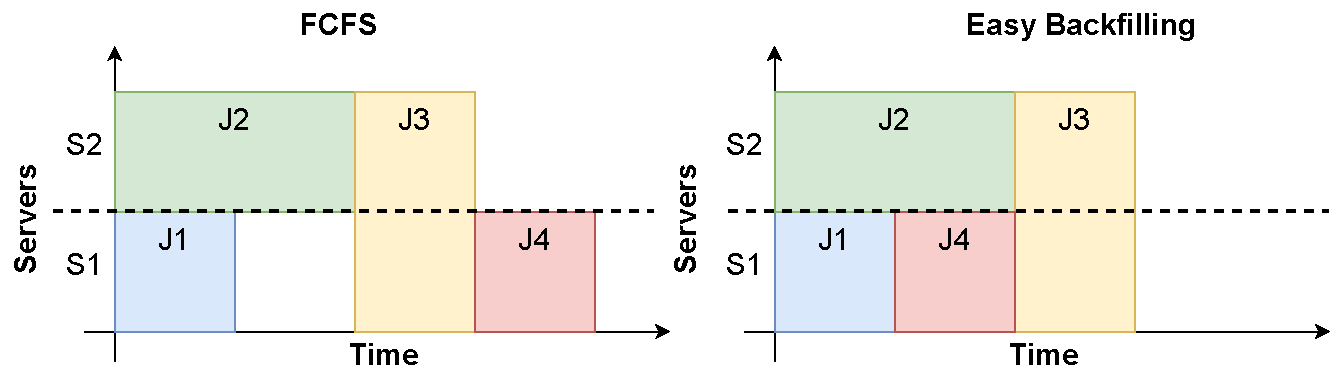
\includegraphics[scale=0.6]{Images/Related_works/backfilling.pdf}
    \caption{Comparison between FCFS and EASY Backfilling scheduling heuristics.}
    \label{fig:backfilling}
\end{figure}

Machine learning is a subfield of artificial intelligence that contains algorithms capable of automatically learning from data and improving performance on specific tasks. In some cases, they emulated the process of human learning. For example, Artificial neural networks simulate the neural network from the human brain. Another example is Reinforcement Learning (RL), which considers the trial-and-error approach, where an agent explores an environment, takes actions, and receives feedback \cite{kaelbling1996reinforcement}. Three components compose an RL model: \textbf{state}, \textbf{action}, and \textbf{reward}. Let's exemplify it by using RL to define the website content. A website can apply RL to define which content to display for the user. The idea is to discover the user's subject preferences (e.g., sports, politics, technology, etc.) The \textbf{state} is the information about the user, such as age, previous subjects read, etc. Using this \textbf{state}, the RL evaluates it and chooses the articles to show to the user. The chosen articles' subjects are the \textbf{actions}. Finally, the \textbf{reward} can be 1 if the user clicked on the article and 0 if the user did not click on it. RL algorithm tries to maximize (in this case) the \textbf{reward}, increasing the number of clicks. Since RL does not know the user's behavior, it tries some articles. The clicked articles reinforce the user's subject preferences. Then, the following process is performed at each decision moment (see Figure \ref{fig:reinforcement}):
\begin{enumerate}
    \item RL receives a state from the environment;
    \item RL verifies which action to take for this state;
    \item RL applies the action in the environment;
    \item The environment returns a reward for this action;
    \item RL uses the reward to calculate the relation between state and action;
    \item The environment goes to a new state, restarting the process.
\end{enumerate}

The RL interacts with the environment in this way several times. RL uses the feedback (reward) to learn which are the best actions for the states. Another important aspect is the exploration-exploitation. Since the RL agent does not know the environment in the early interactions, it starts exploring the different actions in the state. After some interactions, the agent stops the exploration and starts to exploit the actions with higher rewards in the past. Different approaches can be used to model the exploration-exploitation transition, which also depends on the RL algorithm. 

\begin{figure}[!htb]
    \centering
    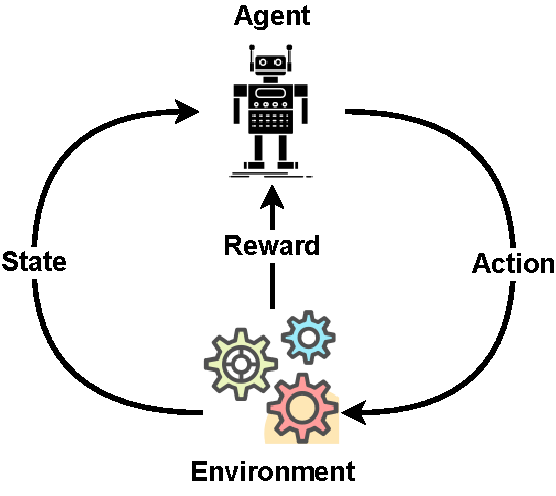
\includegraphics[scale=0.6]{Images/Related_works/Reinforcement_learning.pdf}
    \caption[Agent learning process in an environment]{Agent learning process in an environment. At each step, the agent verifies the actual state and chooses an action. The environment executes the action and returns a reward. The agent learns the reward obtained in that state for that action.}
    \label{fig:reinforcement}
\end{figure}

Metaheuristics are another kind of algorithm to solve hard optimization problems. The "meta" term indicates that they are "higher level" heuristics, different from the problem-specific heuristics \cite{boussaid2013survey}. They are nature-inspired (based on some principles from physics, biology, or ethology). An example is the Genetic algorithm which simulates the evolution and mutation process from biology. Another example is Swarm algorithms inspired by the collective behavior of social insect colonies and other animal societies. Generally, metaheuristics are used to solve problems with no satisfactory problem-specific algorithm \cite{boussaid2013survey}.

Finally, \citeauthor{myerson1991game} defines game theory as ``the study of mathematical models of conflict and cooperation between intelligent rational decision-makers''. Game theory uses mathematical techniques to make decisions in situations with two or more individuals and where the decisions impact the welfare of each individual. Even having the word "game" in its name, it is not only related to recreative activities, and it could be applied to different situations \cite{myerson1991game, osborne2004introduction}. Therefore, like in a game, a set of actions is given to each individual, that needs to make their actions using their interests. The individual's actions return gains or losses (depending on the model) for all "players". This kind of algorithm is known for solving conflict problems.

In this thesis, we apply exact algorithms, greedy heuristics, and machine learning directly in this thesis. A game theory can be applied between offline and online parts (the following section explains its usage). In the offline part, we applied exact algorithms to find optimal solutions. For online, we propose heuristics to solve the specific problem. We also attempted to introduce RL to learn the environment's behavior. Since the online problem needs a fast solution for a specific problem, metaheuristics were not studied.

\section{Datazero2 Project}
\label{sec:datazero2_project}

The Datazero2 project aims to integrate all IT and electrical elements in a feasible architecture \cite{Datazero}. This integration englobes the sizing of all elements (e.g., number of serves, model of wind turbines and solar panels, battery and hydrogen capacity, etc.), the interconnections between electrical and IT devices, power and workload predictions, message format among all elements, and decision processes. Figure \ref{fig:model} presents the architecture of the project. The figure's bottom part illustrates the IT (nodes/servers) and power (battery, hydrogen, wind turbines, and solar panels) elements. All the components (servers, electrical elements, decision modules, etc.) communicate through a Message BUS. On the decision side, it is possible to divide the decision into two main parts: offline and online. Offline consists of IT Decision Module (ITDM), Negotiation Module (NM), and Power Decision Module (PDM). Negotiation is a crucial step in Datazero2 architecture. A renewable-only data center introduces several constraints and decision variables. On the PDM side, it must approximate demand and production while considering long-term storage elements. For example, PDM can provide more power from hydrogen in a case with low renewable generation. However, PDM must evaluate the impact of its actions since the energy of the storage is finite. On the other hand, ITDM maximizes the Quality of Service. Thus, it demands more energy to run more servers at faster speeds. Both PDM and ITDM make their decisions using predictions (weather prediction for PDM and workload prediction for ITDM).

\begin{figure}[!htb]
    \centering
    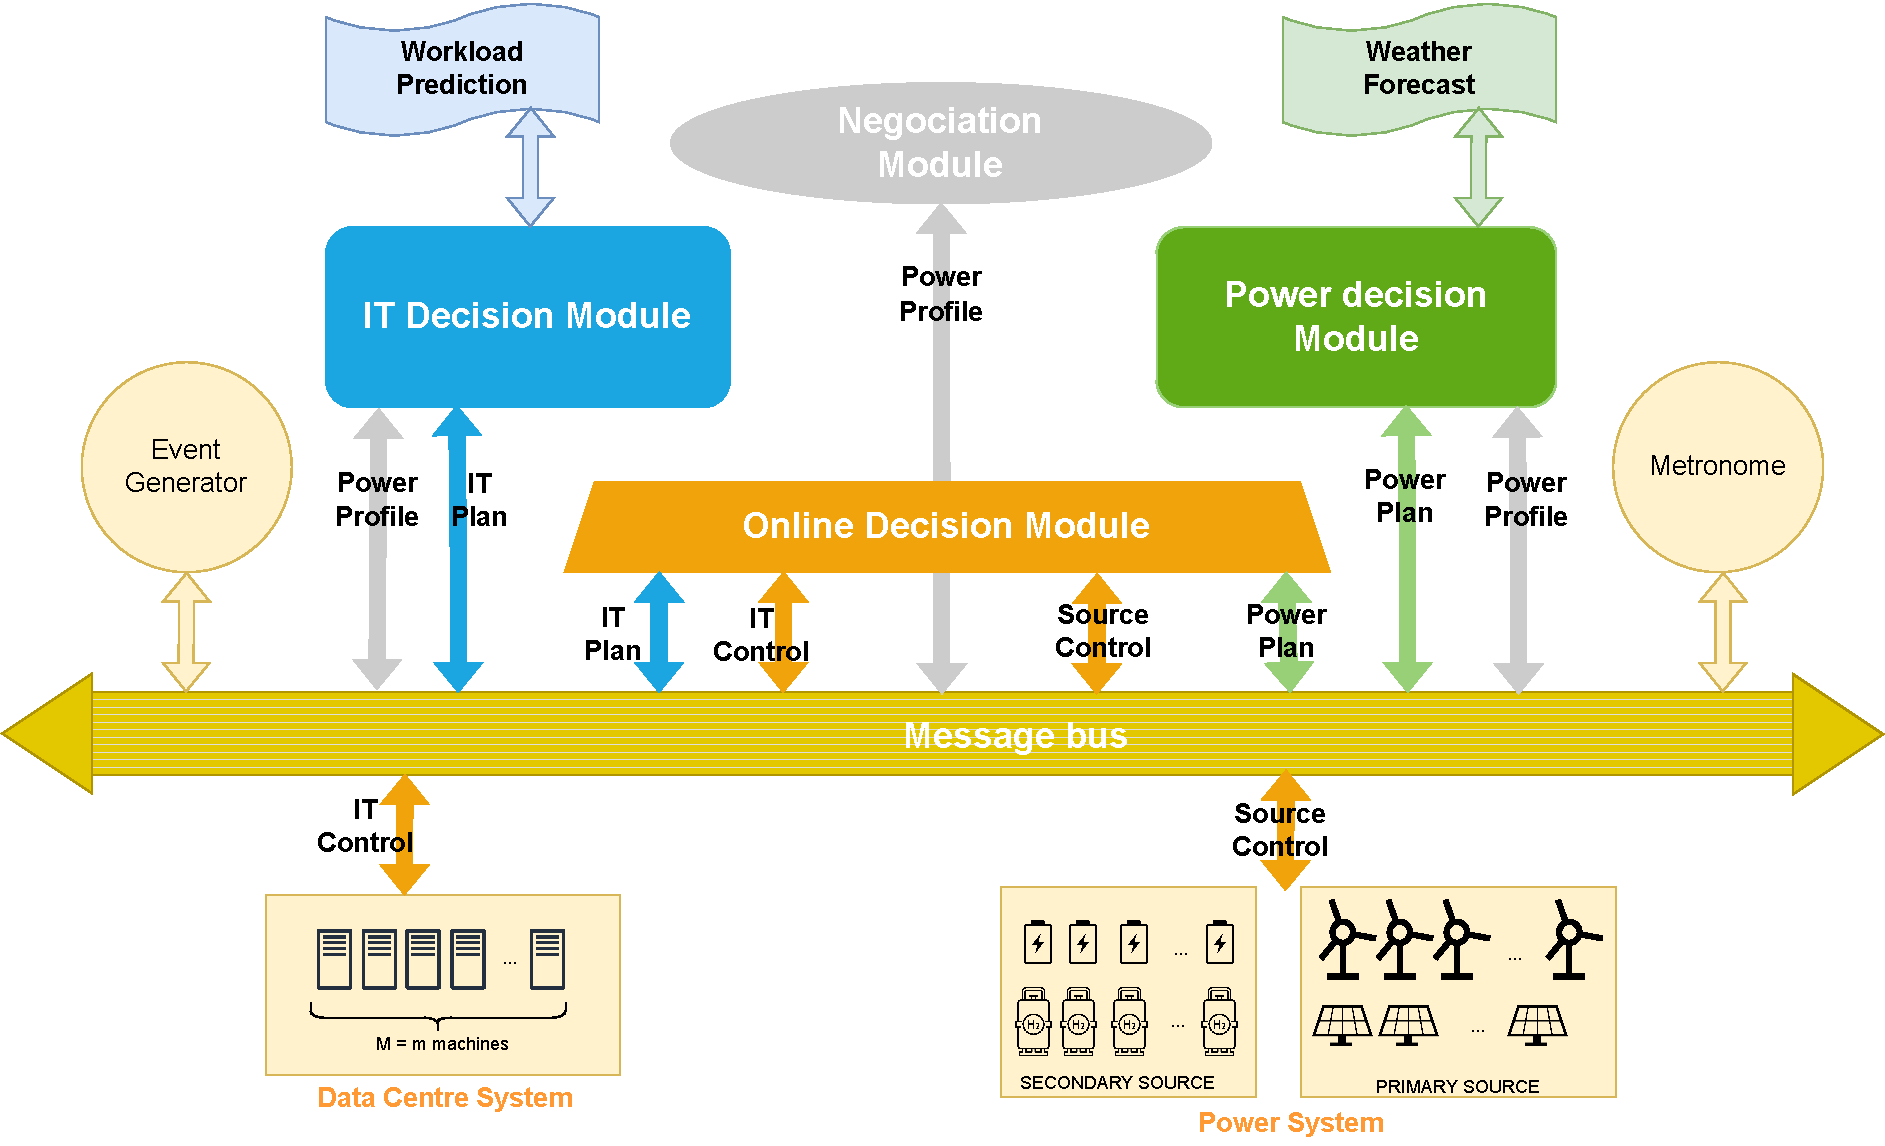
\includegraphics[scale=0.45]{Images/Model/model.pdf}
    \caption[Datazero2 architecture.]{Datazero2 architecture \cite{Datazero}.}
    \label{fig:model}
\end{figure}

NM is between PDM and ITDM, trying to find an agreement. NM works iteratively in several rounds, using a game theory algorithm. On each round, both PDM and ITDM propose a power envelope to NM, considering the objective of each module. A power envelope is a time series of the power production from the sources in a time window. While PDM tries to reduce the power envelope to control the storage, ITDM increases it to run more jobs faster. NM compares both envelope propositions and returns a new one. Then, each module verifies if they can use the proposed power envelope. They run several rounds until both agree or reach a timeout. At the end of the negotiation game, each module creates a plan for the IT and electrical elements, respecting the power profile. ITDM produces the IT Plan and PDM creates the Power Plan. This step ends the offline part. 

The only decision module that works in online mode is Online Decision Module (ODM). This module is the focus of this thesis. It receives both plans from the offline modules. ODM can control all the IT and electrical elements. Besides the plans, ODM also receives through the message BUS the real events, such as power production and job arrival. Therefore, ODM applies the plan, making modifications according to the real events. For example, in a lower power production situation, ODM can reduce IT power usage to match production and usage. The following chapters will explore the algorithms to implement ODM.

\section{Literature Review}
This section presents works to solve the issues related to a renewable-only data center. Several works introduce data centers powered fully or partially by renewable sources. \citeauthor{rostirolla2022survey} propose an extensive survey about the challenges and solutions of renewable sources in data centers \cite{rostirolla2022survey}. The survey highlights the importance of IT and electrical (production and storage) sizing. An overestimated sizing can be too expensive to buy and manage, while an underestimated sizing can not be enough to cope with the workload demand. In this thesis, we do not focus on the sizing, considering that the sizing is known a priori. The survey also indicates open challenges in infrastructure. They present two open challenges: power redundancy and cooling. Power redundancy allows to switch the power provider in case of failure. However, it introduces infrastructure challenges (e.g., failure detection, different redundancy architectures, energy storage architecture, etc.). Several articles study the cooling system of a data center, providing different approaches for controlling the room temperature of the servers. Some solutions include thermal-aware scheduling and free-cooling approaches. Both infrastructure problems are out of our scope. Another aspect is related to geo-distributed data centers. A geo-distributed data center increases server availability by using geographically distributed power production. Even if this is a hot topic, we consider a single data center with local production. 

Finally, the survey also presents some predictions and online decision challenges. The authors indicate that mixing prediction (workload and power production) with online decisions can provide a more robust solution. Also, they highlight the importance of studying the impact of uncertainties in the solution, adding reactiveness in the decision-making. Therefore, we verify the decisions on both offline and online levels for single data centers. Some articles are not renewable only but introduce renewable in the decision process. We divided the articles into three groups: offline only, online only, and mixed decisions. The works are presented in chronological order inside each group.

\subsection{Offline Decisions Only}
\citeauthor{gu2015green} \cite{gu2015green} proposed an Integer Linear Programming for minimizing the carbon emissions of a data center while meeting the scheduling QoS (response time), and considering distributed data centers. Their LP finds the optimal solution to meet a response time constraint, the minimal number of servers, and the best moments to make the server available (e.g., when there is more renewable production). They used an M/M/n model to schedule service requests. They inserted an electricity budget as a constraint. \citeauthor{kassab2017scheduling}, in \cite{kassab2017scheduling}, \cite{kassab2018assessing}, and \cite{kassab2019green}, defined an offline scheduling model to minimize the makespan under power constraints (renewable-only data center). The works were developed in the context of the Datazero project. They proposed heuristics and metaheuristics to find the optimal solution to the NP-Hard scheduling problem. The works \cite{kassab2017scheduling} and \cite{kassab2018assessing} focus only on schedule, maintaining the server availability static (e.g., the server state is previously), while in \cite{kassab2019green}, the authors take a step further, adding server decisions (machines on/off). The server decisions are to turn on servers when needed (and there is power available in the power envelope) and shut down idle servers. All three works ignore power decisions, such as using more or less power from batteries, or online uncertainty.

In \cite{hu2018schedule}, the authors created a weighted average scheduling algorithm (WALECC). This algorithm receives a DAG of a parallel application and defines the job placement. This article is unrelated to renewable energy. However, the problem of a system with energy constraints is similar to a renewable-only data center. WALECC mixes heterogeneous processors with DVFS decisions to find the optimal placement (considering makespan) respecting the energy constraints. WALECC works offline because it knows all the jobs in advance, having the information of each job execution time on each processor/speed. Since it receives the relationship between the jobs through a DAG, it respects the jobs' precedence. \citeauthor{lu2018energy} \cite{lu2018energy} presented a robust optimization for scheduling and power decisions aiming to minimize energy costs. Their scheduling model knows the execution time of each job at different nodes (servers). The authors introduced renewable production uncertainty in the model. Since the uncertainty introduces a random variable, they created a threshold-based algorithm to choose the solution considering the uncertainty distribution. The cost minimization is solved using Linear programming on MATLAB's MOSEK optimization toolbox.

\citeauthor{caux2018optimization} \cite{caux2018optimization} introduced RECO, a Genetic based algorithm. RECO aims to minimize jobs' due date violations in a renewable-only data center. In an offline way, RECO defines the optimal DVFS frequency to run batch jobs and the server states (on/off). Therefore, it works on both scheduling and server configuration. RECO applies a genetic algorithm, creating several scheduling possibilities (pair of job and server) as chromosomes. It applies crossover and mutation, selecting the best-fitted genes. They proposed two fitness functions (to choose the genes). First, a function to reduce the number of due date violations, and the second one uses a weight-based approach, mixing due date and power consumption. The exact processor, frequency, and starting time are assigned using a greedy heuristic. \cite{caux2019phase} is an evolution of \cite{caux2018optimization}, where \citeauthor{caux2019phase}  proposed a new heuristic named MinCCMaxE and a heuristic for degradation. The objective is to maximize the profit from the batches and services execution. Both services and batches are composed of different phases. Services run all the time window duration. On the other hand, MinCCMaxE must find the best placement for batches. MinCCMaxE cross-correlates task and processor loads (both as time series). If it does not find placement (due to power constraints), it delays or degrades the jobs. The degradation step considers the impact on the profit. Both works (\cite{caux2018optimization} and \cite{caux2019phase}) were developed in the context of the Datazero project.

\citeauthor{haddad2019mixed} \cite{haddad2019mixed} modeled a Constraint Satisfaction Problem to define power decisions in a renewable-only data center. This work considers wind and solar as renewable production and battery and hydrogen as energy storage. The objective is to find the power decisions (e.g., battery charge, hydrogen discharge, etc.) that approximate the power produced and demanded. They defined target levels of battery and hydrogen hard constraints. So, the decision variables are battery and hydrogen usage and a relax factor applied to the relationship between produced and demanded. The model considers all losses in power generation, such as battery discharge rate, battery charge/discharge efficiency, hydrogen charge/discharge efficiency, etc. This work is also in the context of the Datazero project. In \cite{gao2020smartly}, the authors proposed a system for matching renewable production and demand. They predicted renewable generation and energy demand using Long Short-Term Memory (LSTM). Renewable production comes from wind turbines and solar panels, using brown energy as a backup. The model uses the result of the predictions to map renewable sources to physical machines. They solved the problem using integer linear programming and Deep Q-Network. Deep Q-Network is an extension of the Reinforcement Learning algorithm Q-Learning. 

\citeauthor{wiesner2022cucumber} \cite{wiesner2022cucumber} created Cucumber, an admission control policy. The authors use probabilistic forecasts to predict power demand (from workload) and production (from renewable sources). Using both predictions, they calculate how much energy is free to use (named freep). The freep is a time series of renewable production minus power demand. Since probabilistic forecasts results in several predictions, they introduced a parameter to tune the forecasts' optimism. Then, they evaluate the freep time series to accept or reject new jobs in an FCFS fashion. They verify if placing a new job using freep capacity would violate the deadline from the other jobs. If so, they reject the new job. The idea is to maximize the peak of renewable production without adding batteries. \citeauthor{yuan2022optimal} \cite{yuan2022optimal} proposed an optimization problem to minimize the operating cost of the entire data center. The data center is powered by renewable energy coming from wind turbines and solar panels, energy storage, and the grid. Their model considers the possibility of selling and buying energy to the grid. For solar and wind turbines, the authors take into account the operation and maintenance costs. They modeled the IT part considering network equipment and cooling system. Similar to other works, they consider batches and services, considering their delay characteristics. 

\subsection{Online Decisions Only}

\citeauthor{aksanli2011utilizing} \cite{aksanli2011utilizing} presented an online heuristic that uses short-term (30 min) forecasts for green energy in the scheduling process. The green energy comes from wind and solar. The scheduler has two queues, one for services and another for batch. Services will run independently of the green energy available, using brown if needed. Then, they predict the green energy available in the next period. Using this prediction, they estimate the number of slots available to run batch jobs. If the number is greater than the currently available slots, they schedule new jobs and spread the remainder to the running ones. If this number is smaller, the scheduler deallocates some jobs (reducing slots, killing, suspending them, or using brown energy). The authors compared their predictive heuristic with a reactive scheduler that allocates servers according to the energy available. Their solution achieves 3 times better green energy usage and reduces the number of canceled tasks up to 7.7 times.

The authors in \cite{sharma2011blink} presented Blink, a renewable-only manager which fastly changes the state (on and off) to meet a power constraint. For example, if the power supply drops by 10\%, blink deactivates the servers 10\% of the time. They propose this manager completely off-grid. However, the applications must have the ability to stop and resume their execution instantaneously, which is not the case in the majority of the applications. They focused mainly on \textit{memcached} applications, a general-purpose distributed memory-caching system. These applications manage a distributed database, answering other client applications. \textit{memcached} applications have very low execution time since they only have to answer the requests with the demanded data. Applying this policy in applications with higher execution times can lead to execution interruption. They focused in maximize the percentage of answered requests (hit rates).

In \cite{goiri2015matching}, the authors proposed a parallel job scheduler, named GreenSlot, for data centers powered by solar energy but using the grid as backup. Their scheduler uses predictions of solar generation to place jobs in the moments with higher production. If it is impossible to place all the jobs in these moments, GreenSlot finds the moments where the grid energy price is lower. GreenSlot saves energy by deactivating idle servers. It creates several slots with the cost. GreenSlot calculates the cost assuming zero for green and the grid price for brown. It assigns penalty costs on slots that cause the job's deadline, avoiding them. The authors indicated some limitations in their work, such as high job rejection or missed deadlines in data centers with high utilization.

\citeauthor{li2016managing} \cite{li2016managing} created a framework named GreenWorks to manage power and server decisions in a data center powered by renewable energy and using battery and grid as backup. They defined a heuristic to manage power generation in four stages. Stage I is when renewable generation is enough to ensure full-speed server operation. In this stage, the renewable production excess is stored in the batteries. Stage II is active when the production is inadequate to provide the power demanded. Here, the heuristic balance between discharging the battery and impacting the jobs (through DVFS). If this stage is not enough to handle the power mismatch, the system enters stage III. In this stage, GreenWorks tries to decrease load power more, use UPS energy if it has power, and, the last resource, it use the grid. They only use power from the grid for the same amount of energy that they exported previously. So, they accumulate a budget of net green energy exported. If it is not enough, stage IV shuts down the servers. GreenWorks does not use predictions and relies on the first-come-first-serve (FCFS) scheduler.

The authors in \cite{li2017balancing} created an opportunistic scheduling heuristic. This heuristic tries to minimize brown energy usage by mixing batteries and solar production. The heuristic takes into account services and batches. When the energy consumption is higher than the solar supply, they suspend batch jobs and consolidate the VMS, switching off the servers. The scheduler takes energy from the battery before going to the grid. Just after the batteries dry, it starts to consume brown energy. They implemented a First Fit Decreasing (FFD) scheduling algorithm. \citeauthor{grange2018green} \cite{grange2018green} proposed an algorithm named Attractiveness-Based Blind Scheduling Heuristic (ABBSH). ABBSH introduces a negotiation model for electrical and IT systems, where both know only their own model. Negotiation helps to deal with different objectives. For example, the objective of the electrical system is to reduce brown energy usage, while IT is to respect the System Level Agreement (SLA) criteria. Both calculate a normalized metric named attractiveness. This metric represents the quality of a given proposal. So, for each job, it calculates the attractiveness of its placement in the IT and electrical context. Then, a function defines, among all possible placements, which one has the best attractiveness. The authors select the best attractiveness using a simple weighted sum of both (electrical and IT), a weighted sum of the hyperbolic sinus of both, or a fuzzy-based one. In this work, the authors consider the electrical part as a black box without making power decisions.

\citeauthor{haghshenas2020infrastructure} \cite{haghshenas2020infrastructure} developed a heuristic aiming to minimize energy costs. The energy cost (from the grid) is the IT and cooling usage minus solar generation. This heuristic considers services and batches. It always schedules the services in the FIFO approach. It finds the best moment to place batches using best-fit and considering solar production and energy price. Even online, the authors assume knowing all the jobs for the next period. They used solar production predictions to make decisions for the next time slot. They consider the possibility of selling solar production to the grid. They do not consider power on/off transitions, assuming the IT energy consumption is zero when the servers are not running jobs. Finally, the authors updated their algorithm, adding a simplified battery model. The battery will store the surplus solar generation to use later, reducing the energy cost. \cite{nayak2021efficient} proposed an online heuristic to schedule jobs in servers. The main objectives are to minimize the makespan, energy cost, and overall cost and maximize renewable usage. The authors separated the heuristic into three phases. First, they estimated the completion time and cost for the execution of a user request on each data center. The cost considers if the data center is powered by renewable or non-renewable. The second phase calculates the fitness value, normalizing completion time and cost. Finally, the last phase takes the data center with higher fitness to place the user request. The work considers that all the data centers are available all the time (using renewable or not).

In \cite{he2022online}, \citeauthor{he2022online} created an online scheduling heuristic to minimize the energy cost of a data center called ODGWS (Online workload Scheduling algorithm with Delay Guarantee). The authors take into account solar, wind, and grid energy. They simplified the job description to be the power requested at each time step by services and batches. The scheduler must deliver the services' power requested in the same step that they arrive. On the other hand, the scheduler can delay the batches' power demand until a fixed time horizon. So, even if the authors named their algorithm workload scheduling, the decisions are which source to use to provide the energy to the jobs. They do not consider the placement problem (e.g., which server will receive the jobs). Besides, they assume that the servers are available all the time. Their problem is a constrained stochastic problem solved by dynamic programming, but they translated it into an online heuristic, which can work without knowing future events.

\citeauthor{peng2022energy} designed REDUX3 an energy management system with a renewable-aware scheduler. REDUX3 uses energy from different sources, such as wind turbines, solar panels, the grid, diesel generators, and batteries. The system focuses on batch tasks, allowing them to postpone jobs to match production and demand. They added the grid to deal with uncertainties. They created three energy states: Outage Case, Stable Case, and Fluctuate Case. An Outage Case is when the renewable supply is at the minimum, a Stable Case is when the renewable supply exceeds the maximum level, and a Fluctuate Case is when the previous energy state was Outage Case but is stable now. In addition, they introduced three key components. First, the scheduling window module defines the number of available processors according to the energy case. Second, the scheduling algorithm uses a backfilling algorithm to place the jobs in the available processors. This scheduler receives a job priority, considering it in the decision process. Finally, they do a job power profiling, providing data to create a job power model.

In \cite{liu2023online}, the authors defined an online energy-aware scheduling algorithm using deep reinforcement learning. The main idea is to use the grid power when the carbon emission rate is lower. They used a DAG to define the different tasks of a batch job. The DAG indicates when a task can start (e.g., task 2 can run after task 1 is finished). A typical reinforcement learning algorithm has three key elements: state, actions, and reward. The state in this article is given by server usage, task queue, electricity price, and emission rate. The task queue contains only the tasks ready to run, considering the job's DAG. The actions are the tuple of task and server, considering the feasibility of this tuple (if a server can not receive the task, it is not a feasible action). Finally, the reward is carbon, cost, and QoS. They do not introduce server decisions, so the servers are always available.

\subsection{Mixed decisions}

The only work that mixed offline and online decisions is \cite{venkataswamy2023rare}. In the offline part, the authors predict renewable energy production. They use these predictions, energy storage, and brown energy to fix the number of resources. After that, online makes the scheduling decisions considering the offline server configuration. They created a deep reinforcement learning algorithm to define the jobs to run. The state is composed of tuples containing both the resource availability and the array of job metadata. The job metadata includes the price that the user is willing to pay, QoS, expected finish time, duration, and resource requirements. The actions are which job run, suspend a job, or do nothing. So, they can suspend a job, placing a job with a higher price first. This suspended job will run later. Finally, the reward is the total value obtained by running the jobs respecting the QoS. The authors indicate that power decisions would transform their problem into a multi-criteria optimization problem. These power decisions include changing battery usage and selecting power sources. They claimed that this multi-criteria optimization is future work. They evaluated the impact of the power supply intermittence on the algorithm, but DRL does not consider it in the model.

\subsection{Discussion and Classification of the Literature}
Table \ref{tab:related_works} presents all the works presented in the previous section. We classified them considering 5 criteria:

\begin{itemize}
    \item \textit{Objective}: It describes what each article aims to optimize;
    \item \textit{Electrical infrastructure}: It synthesizes the power sources, such as solar panels, wind turbines, batteries, hydrogen, diesel generator, and the grid;
    \item \textit{Offline decision}: The type of decisions in offline way. We classify these decisions into scheduling, server, and power decisions. Scheduling decisions focus on placing the jobs, deciding the order, rejecting jobs, selecting the servers, etc. Server decisions are the decisions about the availability of the servers, such as server state (on/off) or speed (DVFS). power decisions define power usage (e.g., charging/discharging batteries);
    \item \textit{Online decisions}: Same as offline decisions, but in online mode;
    \item \textit{Method}: The method used to solve their problem (e.g., Heuristic, Exact algorithm, etc);
\end{itemize}

It is possible to notice that several works introduce renewable energy in data centers environment. As mentioned before, renewable sources provide clean but intermittent power. The majority of works add a connection to the grid, aiming to reduce the impact of the intermittence. However, these approaches maintain the brown energy dependency. Some of the works with the grid have as their objective to minimize energy costs, adding the possibility of selling energy to the grid. This could lead to a solution where selling energy is more attractive than running jobs due to price fluctuations. As presented in this chapter, migrating entirely to renewable sources is mandatory. Several works without grid connections are from the Datazero project. They are pertinent works and are the base of this thesis. The only outside Datazero no-grid works are from \citeauthor{wiesner2022cucumber} and \citeauthor{sharma2011blink}. The first one focuses on using the peak of renewable sources to schedule new jobs. In our work, and other works from the literature \cite{li2016managing, li2017balancing, haddad2019mixed, haghshenas2020infrastructure, nayak2021efficient, peng2022energy, yuan2022optimal, venkataswamy2023rare}, these peaks are stored in energy storage. These energy storages (e.g., batteries or hydrogen) help to smooth the RES intermittence but introduce another decision level. The work from \citeauthor{sharma2011blink} deals with web service applications by blinking (deactivating/activating) the servers. This behavior demands small applications (low execution time) or applications with the possibility of fastly stopping and resuming their execution. 

Usually, the works with energy storage only apply it as an energy cache. So, they can dry or overflow these resources, without good management. Maintaining the state of charge of batteries between a narrow range can increase the battery's life. Only \citeauthor{li2016managing} consider good battery decisions to maximize the battery life span. However, the authors balance using the battery or buying energy from the grid. Another important aspect of battery management is related to mixing short, and long-term decisions. In short-term decisions (online), it could dry the battery to maximize the QoS. However, the battery is finite and this behavior could lead to future QoS degradation (e.g., drying the battery in the short-term would reduce battery usage in the future, decreasing the power available to IT servers).

Table \ref{tab:related_works} also highlights that the majority of the previous works only focus on one side of the decision process. Sometimes they make offline decisions considering knowing all the future events or using predictions. These works focus on finding an optimal solution for the problem. However, the uncertainties of a renewable-only data center demand a reaction when the solution is not feasible in reality. Another possibility is working online entirely, reacting to events or using fast predictions. In this case, we lose the long-term aspects. For example, it is simple to maximize the number of jobs running in a renewable-only data center if the system dries the energy storage. However, in the big picture, this behavior leads to problems in the following days. \cite{venkataswamy2023rare} is the only work aggregating decisions on two levels, but with a simple offline server configuration. They create this configuration using power from the grid, and they do not change battery usage to react to actual production.

This thesis aims to provide algorithms to integrate both offline and online decisions. While the offline creates a plan considering long-term, online reacts and adapts this plan. To the best of our knowledge, there are still no approaches integrating both sides to make better decisions. Furthermore, we introduce three levels of decisions, considering server states, job scheduling, and power decisions. Mixing all these aspects allows us to follow the long-term plan while improving QoS. Finally, we focus on batch jobs. The services appear in some works as a constraint, since they do not make big decisions about them (e.g., some authors use brown to meet service QoS).

\begin{landscape}

\begin{table*}[htp]
\centering
\caption{Summary of characteristics for existing renewable data center scheduling works.}
\label{tab:related_works}
\begin{tabular}{m{3cm}|m{0.8cm}|m{3cm}|m{3.2cm}|m{3cm}|m{3cm}|m{3cm}}
\hline
Article & Year & Objective & Electrical infrastructure & Offline decisions & Online decisions & Method \\ \hline\hline
\citeauthor{aksanli2011utilizing} \cite{aksanli2011utilizing} & 2011 & Maximize green energy usage & Solar panels, wind turbines, and grid & - & Server and Scheduling & Heuristic \\ \hline
\citeauthor{goiri2015matching} \cite{goiri2015matching} & 2015 & Maximize green energy usage and reduce grid energy cost & Solar panels and grid & - & Server and Scheduling & Heuristic \\ \hline
\citeauthor{gu2015green} \cite{gu2015green} & 2015 & Minimize carbon emissions & Solar panels, wind turbines, and grid & Server, Scheduling, and Power & - & Exact algorithm \\ \hline
\citeauthor{li2016managing} \cite{li2016managing} & 2016 & Balance QoS, battery life span, and average backup time & Wind turbines, batteries, and grid & - & Server, Power & Heuristic \\ \hline
\citeauthor{kassab2017scheduling} \cite{kassab2017scheduling} & 2017 & Minimize makespan and flowtime & Solar panels and wind turbines & Scheduling & - & Heuristic \\ \hline
\Citeauthor{li2017balancing} \cite{li2017balancing} & 2017 & Maximize green energy usage & Solar, batteries, and grid & - & Server, Scheduling, and Power & Heuristic \\ \hline
\citeauthor{kassab2018assessing} \cite{kassab2018assessing} & 2018 & Minimize makespan and flowtime & Solar panels and wind turbines & Scheduling & - & Metaheuristic \\ \hline
\citeauthor{grange2018green} \cite{grange2018green} & 2018 & Minimize grid energy and respect QoS & Solar and grid & - & Server and Scheduling & Heuristic \\ \hline
\end{tabular}
\end{table*}

\begin{table*}[htp]
\centering
\begin{tabular}{m{3cm}|m{0.8cm}|m{3cm}|m{3.2cm}|m{3cm}|m{3cm}|m{3cm}}
\hline
Article & Year & Objective & Electrical infrastructure & Offline decisions & Online decisions & Method \\ \hline\hline
\citeauthor{hu2018schedule} \cite{hu2018schedule} & 2018 & Minimize makespan under energy constraints & - & Scheduling & - & Heuristic \\ \hline
\citeauthor{lu2018energy} \cite{lu2018energy} & 2018 & Minimize energy cost & Solar panels and grid & Scheduling and Power & - & Exact algorithm \\ \hline
\citeauthor{caux2018optimization} \cite{caux2018optimization} & 2018 & Maximize QoS under power constraints & Solar panels and wind turbines & Server and Scheduling & - & Metaheuristic and heuristic\\ \hline
\citeauthor{caux2019phase} \cite{caux2019phase} & 2019 & Maximize profit under power constraints & Solar panels and wind turbines & Server and Scheduling & - & Heuristic\\ \hline
\citeauthor{haddad2019mixed} \cite{haddad2019mixed} & 2019 & Match power demand and production & Solar panels, wind turbines, batteries, and hydrogen & Power & - & Exact algorithm \\ \hline
\citeauthor{gao2020smartly} \cite{gao2020smartly} & 2020 & Match power demand and production minimizing QoS violations & Solar panels, wind turbines, and grid & Power & - & Exact algorithm and machine learning \\ \hline
\citeauthor{haghshenas2020infrastructure} \cite{haghshenas2020infrastructure} & 2020 & Minimize energy cost & Solar panels, batteries, diesel generator, and grid & - & Scheduling, and Power & Heuristic \\ \hline
\citeauthor{nayak2021efficient} \cite{nayak2021efficient} & 2021 & Minimize makespan, energy consumption, and overall cost, and maximize renewable usage & Not specified (renewable and non-renewable without battery) & - & Scheduling & Heuristic \\ \hline
\end{tabular}
\end{table*}

\begin{table*}[htp]
\centering
\begin{tabular}{m{3cm}|m{0.8cm}|m{3cm}|m{3.2cm}|m{3cm}|m{3cm}|m{3cm}}
\hline
Article & Year & Objective & Electrical infrastructure & Offline decisions & Online decisions & Method \\ \hline\hline
\citeauthor{he2022online} \cite{he2022online} & 2021 & Minimize energy cost & Solar panels, wind turbines, and grid & - & Power & Heuristic \\ \hline
\citeauthor{peng2022energy} \cite{peng2022energy} & 2022 & Minimize energy cost & Solar panels, wind turbines, batteries, diesel generator, and grid & - & Server, Scheduling, and Power & Heuristic \\ \hline
\citeauthor{wiesner2022cucumber} \cite{wiesner2022cucumber} & 2022 & Maximize renewable excess energy usage & Solar panels and wind turbines & Scheduling & - & Heuristic \\ \hline
\citeauthor{yuan2022optimal} \cite{yuan2022optimal} & 2022 & Minimize energy cost & Solar panels, wind turbines, batteries, and grid & Power & - & Exact algorithm \\ \hline
\citeauthor{liu2023online} \cite{liu2023online} & 2023 & Minimize the energy consumption cost and carbon footprint & Grid & - & Scheduling & Machine learning \\ \hline
\citeauthor{venkataswamy2023rare} \cite{venkataswamy2023rare} & 2023 & Maximize job value (revenue) & Solar panels, wind turbines, batteries, and grid  & Server & Scheduling & Machine learning \\ \hline

\end{tabular}
\end{table*}

\end{landscape}
% \begin{itemize}
%     \item Article;
%     \item Year;
%     \item Objective;
%     \item Electrical infrastructure (solar, wind, battery, grid, etc);
%     \item Offline decisions (Scheduling, Power, Server, both);
%     \item Online decisions (Scheduling, Power, Server, both).
% \end{itemize}
% Scheduling means server on/off and job scheduling

\section{Conclusion}

This chapter focused on presenting the motivations and fundamentals for understanding this work. We started explaining the context, going from global warming to the role of renewable-only data centers on climate change. Then, we detailed the several elements that compose a renewable-only data center. Finally, we described the different sources of uncertainty, presenting some classes of algorithms to deal with them. In the second part of this chapter, we showed different works on applying renewable sources in data centers. We clarify the different approaches, highlighting the gaps in the state-of-the-art.